\chapter{基于模型匹配的机器人辅助人体坐立运动时间自适应}
人类从坐姿到站姿的转换是日常生活中常见的动作,涉及复杂的人体感知和执行机制。具有站立辅助功能的机器人、智能轮椅和人形辅助机器人对帮助失能或半失能人群完成坐立动作起着至关重要的作用。被辅助人的坐立完成时间具有随机性,对于被辅助对象完成运动的交互意图感知也是是设计优化控制器的难点。本章研究了在机器人辅助坐立控制中,如何基于坐立运动轨迹观测在线预测被辅助对象意图完成运动的时间。虽然基于数据驱动的方法在多项预测任务中效果显著,但在仍然在难以获得大量人体运动数据的情况下实时。此外,考虑到康复辅助机器人必须保证系统的安全,相关算法的可解释性变得尤为重要。针对这些问题,围绕一个共享自主框架中的轨迹优化问题,本章提出了一种基于系统参数辨识的运动时间预测方法。理论分析表明,此方法通过单一运动示教轨迹即可预测运动速度,可有效提升数据使用效率。

\section{研究动机}
坐立活动是人类日常生活中最常见且基本的动作之一,要完成这一动作,需要依赖足够强壮且健康的下肢肌肉群来执行一系列复杂的生理活动。然而,随着我国人口老龄化的不断加深,相关研究表明即使是健康的老年人,也可能因为频繁重复的膝关节运动导致下肢关节功能和运动机能退化\cite{heidariKneeOsteoarthritisPrevalence2011},此外还有大量的膝无力和患有各种慢性疾病或残疾人存在站立转移困难的问题。在生物工程和康复机器人领域,存在诸多关于设计和制造用于坐立助力的功能性辅助机器人的研究。近年来随着人工智能技术和通用人形机器人的发展,智能化程度更高和约束更少的坐立辅助机器人成为研究的主要方向。例如使用通用的移动机械臂平台进行站立辅助,其相较于定制化设备可以满足不同活动的辅助,更具经济优势\cite{liIntegratedApproachRobotic2021}。然而,这对辅助机器人对不同的被辅助对象的适应性提出了更高的要求。一个完整的坐立运动过程通常包含两个不同的阶段,第一个阶段为上身姿态调整,而第二个阶段为下肢发力完成站立。例如,在坐姿起床前,被辅助对象需要调整重心,以便他/她能够成功地站起来。因此,为了保证性能和安全,在机器人运动辅助中,机器人对于人类的意图理解对于实现机器人的自适应运动规划与控制起着重要的作用,因为人类不仅是需要辅助的人,也是自然试图领导机器人运动的主人。其中存在的典型人机交互不确定性因素包括改变站立速度,或因突然改变决定而坐下来等等。目前已有部分研究针对坐立运动辅助的交互意图进行了研究。例如在研究\cite{liIntegratedApproachRobotic2021}中,作者使用了一个长短时记忆网络网络估计了运动时间意图特征,并将其集成在了一个优化控制框架中。此外,也有研究使用最大后验估计对人体运动动态特征进行估计\cite{romanoCoDyCoProjectAchievements2018}。

\begin{figure}[htb]
    \centering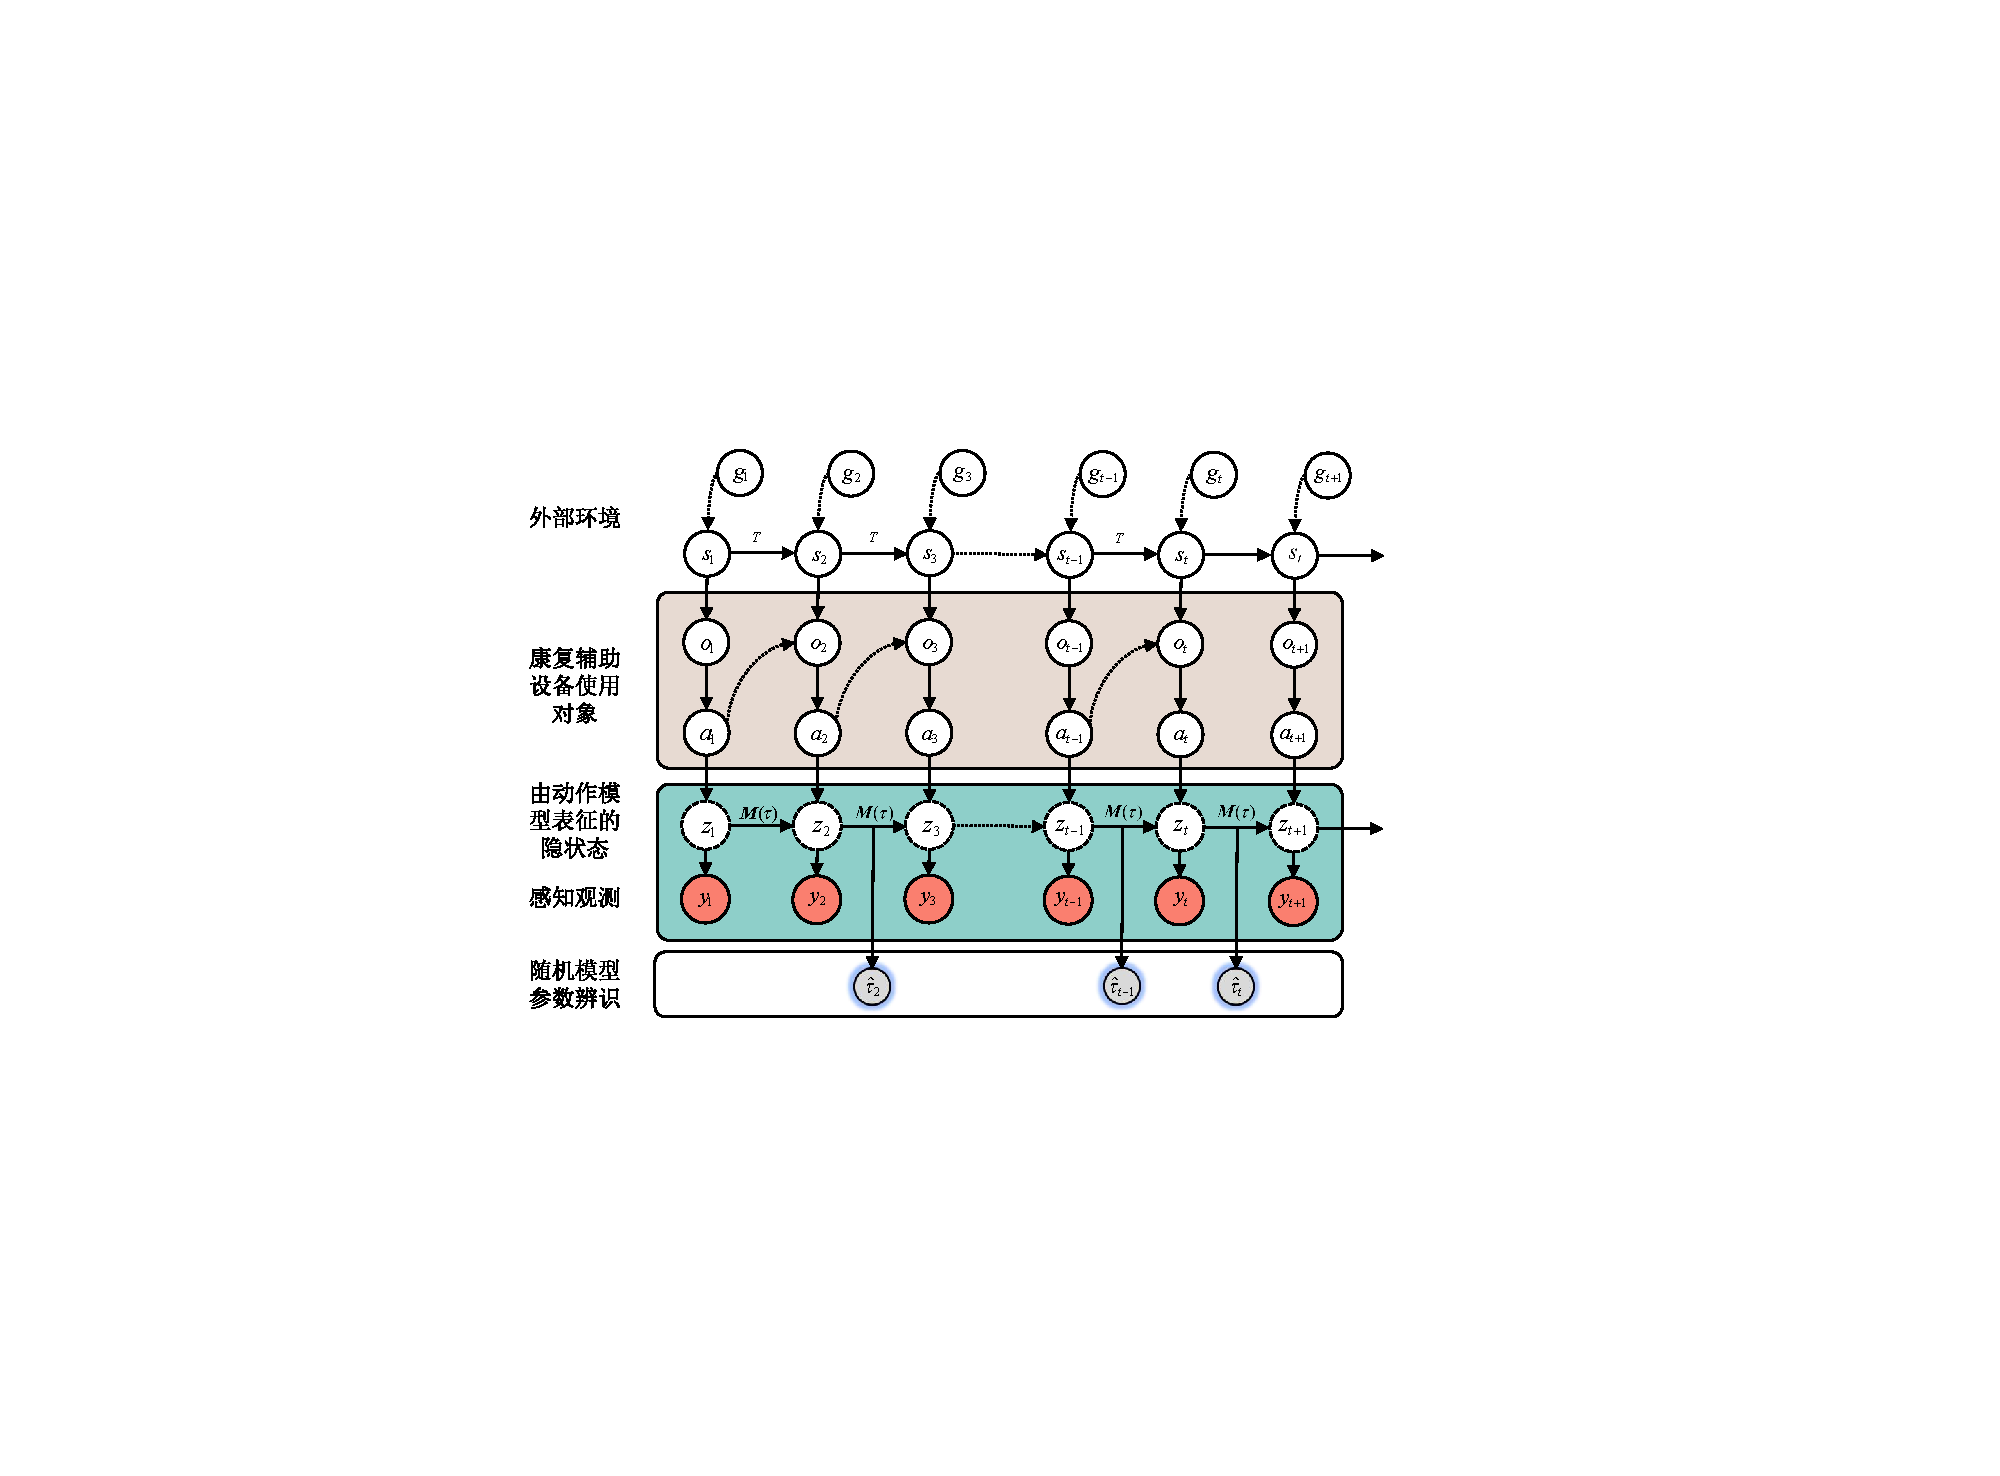
\includegraphics[width=0.8\textwidth]{figures/4-Fig-Intro.pdf}
    \caption{本章所使用的处理交互不确定方法的概率图模型}
    \label{fig:4-Intro}
\end{figure}

完成人由坐到站的时间不同会影响运动过程中的稳定性、肌肉活动、舒适度、能量消耗和运动控制等多个方面。为了确保安全和舒适,站立辅助机器人应当适应使用者由于身体状况和能力不同导致的多样化运动时间。目前关于人类完成站立运动时间意图的在线估计的研究还较少,已有的运动意图估计研究大多基于数据驱动,通过采集大量的运动数据建立意图推断模型,数据利用率较低。然而人类使用不同速度完成站立运动的关节运动轨迹在空间上的拓扑结构是相似的。利用参数化的轨迹模型对人体下肢运动进行建模表征,可以将坐立运动过程中的关节运动时间意图推理看作为一个参数辨识任务,进而设计意图推断方案将会大大提高数据的利用率。第二章已经对于动态运动基元进行了分析和介绍,其中离散型动态运动基元可以通过时间常数对一个标准的点到点轨迹进行缩放,适合用于表征人体坐立动作。因此,本章首先基于离散动态运动基元模型对一组标准的人体坐立运动轨迹进行了参数化建模表征,在此基础上通过考虑人机交互过程中的不确定性因素对离散动态运动基元模型进行了概率化处理,并基于期望最大化算法就运动时间意图推断方法进行了研究。此外,所提出方法可实现在运动中根据当前积累的观测数据进行连续的意图估计并提供估计结果的置信度量化指标,因此其可集成于一个共享自主系统,实现辅助机器人轨迹的在线优化控制或变刚度阻抗控制。
\section{自适应辅助轨迹优化框架}  
连续的交互意图估计是站立辅助机器人自适应辅助轨迹优化中的一个重要环节。在本节,就机器人辅助坐立运动过程中的人机耦合动力学,以及轨迹优化方法进行了介绍。
\subsection{坐立辅助人机耦合动力学模型}  
作为一种简化的人体生物力学模型,三重倒立摆模型在人机混合系统中得到了广泛的应用。图\ref{fig:4-1}给出了基于三重倒立摆模型的人体坐立运动结构图,本章研究通过保留下肢髋、膝、踝3个关节以及足、小腿、大腿和躯干(上身和头部)4个刚体在矢状面的运动构建并分析了人体在坐立过程中的动力学模型。其中,踝关节、膝关节、髋关节的扭矩被用来控制模型的运动,并且对这三个关节的运动轨迹的观测也被用于意图推断。来自辅助机器人的辅助力作用于躯干,通过欧拉-拉格朗日方法可以推导出站立辅助过程的人机耦合动力学方程如下:
\begin{equation}
    \mathbf{H}(\theta) \ddot{\theta}+\mathbf{C}(\theta, \dot{\theta})+\mathbf{G}(\theta)=\tau+\tau_{ext}=\tau_{tot}
    \label{eq:4-1}
\end{equation}
其中$\mathbf{H}(\theta)\in \mathbb{R}^{3\times 3}$是正定的对称惯性矩阵,$\mathbf{C}(\theta, \dot{\theta})\in \mathbb{R}^3$为科里奥利力和向心力矢量,$\mathbf{G}(\theta)\in \mathbb{R}^5$为重力向量。$\theta \in \mathbb{R}^3$ 代表着踝关节($\theta_1$), 膝关节($\theta_2$), 髋关节($\theta_3$)三个关节角度的向量。$\tau \in \mathbb{R}^3$为人体自主运动产生的关节扭矩而$\tau_{ext} \in \mathbb{R}^3$为辅助机器人对被辅助对象在笛卡尔空间施加的外力在关节空间产生的相应扭矩。考虑到外力$F\in \mathbb{R}^m$为施加于人体模型上特定点$k$的一个维度为$m$的外部广义辅助力向量,设与该点相关联的雅可比矩阵为$J_k(\theta)\in \mathbb{R}^{m\times 3}$,则由机器人辅助作用于上身躯干的力量产生的相应关节扭矩为:
\begin{equation}
    \tau_{\text {ext}}=\mathbf{J}_k^T(\theta) F
    \label{eq:4-2}
\end{equation}
关于动力学方程中的矩阵参数确定,在实验中可以直接测量每个人的身高和体重,而每个身体部分的运动学和动力学参数无法直切确定,因此关于不同参与者的各肢体动力学参数的选择可以通过一个标准参数表进行计算\cite{tozerenHumanBodyDynamics2000}。

\begin{figure}[htb]
    \centering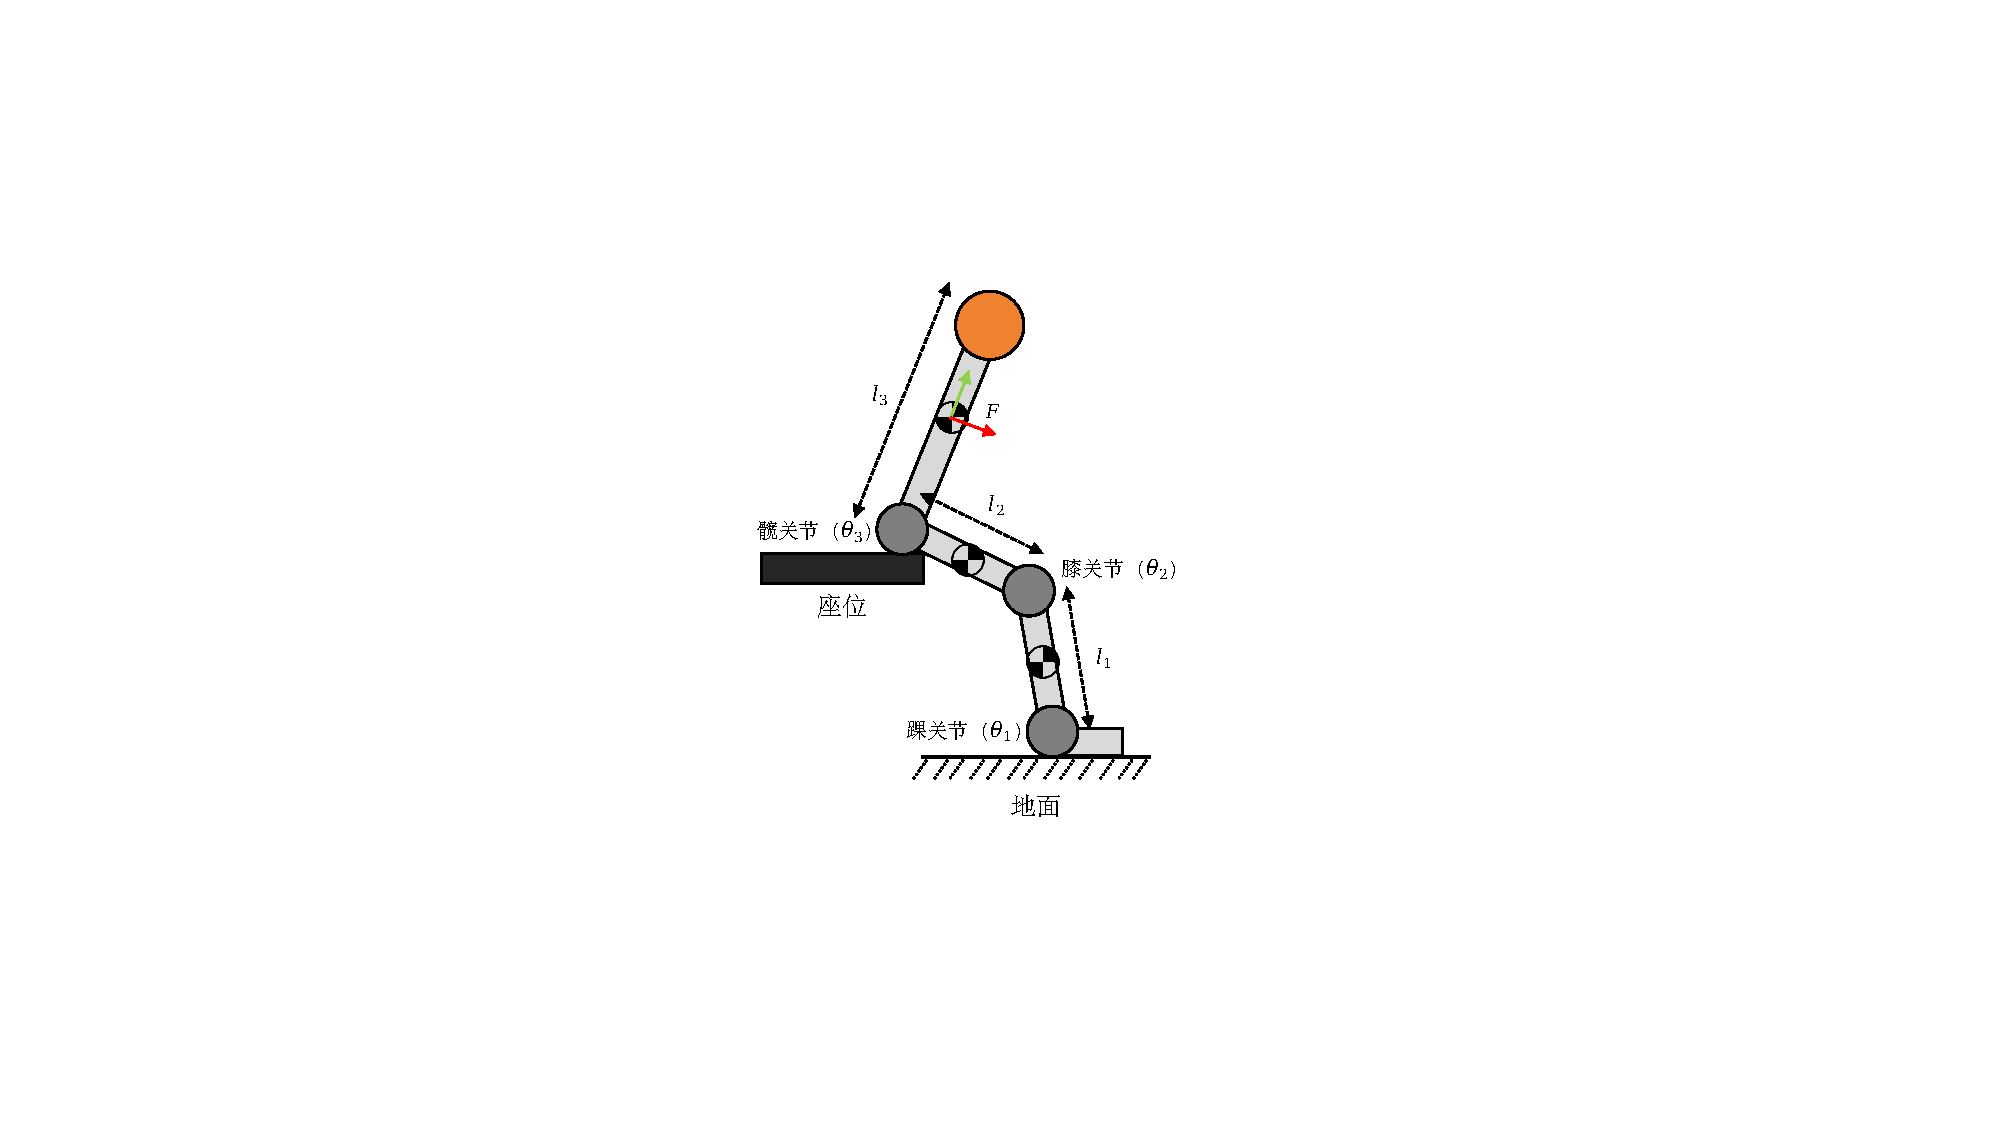
\includegraphics[width=0.4\textwidth]{figures/4-Fig-1.pdf}
    \caption{三连杆人体模型}
    \label{fig:4-1}
\end{figure}
\subsection{基于共享自主的轨迹优化策略}
一个机器人坐立辅助的最优控制问题可以表述如下:在$t=0$时刻,关节速度为零的人保持静止的坐姿在座位上为初始状态,期望的最终状态为在$t=T$时刻关节速度为零的稳定站立状态。坐立辅助机器人的轨迹优化主要目标是找到一个控制律$τ_∗= π(x,t)$,保持在机器人关节转矩限制以及其他边界条件时,辅助人体系统平稳地从初始状态过渡到最终状态的状态,同时最小化给定的成本函数。在定义优化问题的成本函数时,通常可以从三个方面考虑:用户能量消耗、运动和控制的平滑性、平衡保持。其中最小化能量消耗是最为常见和有价值的优化目标,可以通过类似于式\ref{eq:4-3}中的人体能量消耗项$C_{pwr}$来实现的。此外能量消耗损失函数也可以从骨骼肌肉模型的角度来设计,通过结合肌肉激活模型可以更深层次地优化特定肌肉的能量消耗\cite{kumarPredictingSittoStandAdaptations2022}。平滑控制可以通过类似于式\ref{eq:4-4}的关节角加速度损失项$C_{smooth}$来实现的,此外还可以设计用于保持平衡的损失函数等。
\begin{equation}
    C_{pwr}(\tau(t))=|\tau(t)|_{W_{pwr}}^2
    \label{eq:4-3}
\end{equation}
\begin{equation}
    C_{smooth}(x(t))=|\dddot{\theta}(t)|_{W_{smo}}^2
    \label{eq:4-4}
\end{equation}

在设计了相关的损失项和约束项后,可以将他们合并写成一个STS转移的优化目标函数,其中$\boldsymbol{\phi}_{final}$为最终状态损失项,用于控制站立时的关节运动速度为0且保持稳定。每项损失项的权重$W_i$通常由经验设定或由其他优化方法设定:
\begin{equation}
    \boldsymbol{\phi}_{total}=\boldsymbol{\phi}_{final}(\boldsymbol{x})+\int_0^T\left(\sum_{i=1}^6 W_i \boldsymbol{C}_i\right) dt
    \label{eq:4-5}
\end{equation}

在式\ref{eq:4-5}中,优化目标中与状态相关的损失项由一个关于时间的从$t=0$到$t=T$的积分计算得到,其中$T$为完成一个STS动作的时间长度。在相关研究中,一般使用固定的任务完成时间参数计算损失项,通过实验预估或计算平均的STS动作时间进行离线轨迹优化。然而,由于每个被辅助对象的能力不同,导致其在辅助应用中每次完成动作的时间是不确定的。若要实现一个基于优化控制器的在线轨迹规划算法,对于动作完成时间$T$的在线估计不仅仅关系到损失函数的计算,更加体现了机器人对于被辅助对象人机交互不确定性的适应能力。因此,针对该问题,如图\ref{fig:4-2}所示在本章中,意图推理可以通过一个共享自主框架融合到上述的轨迹优化问题中。其中交互意图推理模块通过视觉观测被辅助对象下肢的三个关节的实时角度,在线估计坐立任务完成时间$\hat T$并给出当前估计的置信度$b$。则优化目标积分时间$T$可以通过一个共享自主系统计算:

\begin{equation}
    T=\alpha_b \hat T + (1-\alpha_b)T_{def}
    \label{eq:4-6}
\end{equation}
由于在观测数据较少时无法准确估计可靠的持续时间,因此引入一个预定义的坐立运动完成时间$T_{def}$为基础时间,该参数可通过经验设置以保证机器人的基本工作能力。混合权重$\alpha_b \in [0,1]$为一个关于坐立运动完成时间预测置信度$b$的函数,当置信度较高时$\alpha_b \rightarrow 1$,反之$\alpha_b \rightarrow 0$。通常,随着观测数据的增多对于意图估计的置信度会更高,进而使得对于积分时间长度的估计更加接近预测值而不是预定义值。

\begin{figure}[htb]
    \centering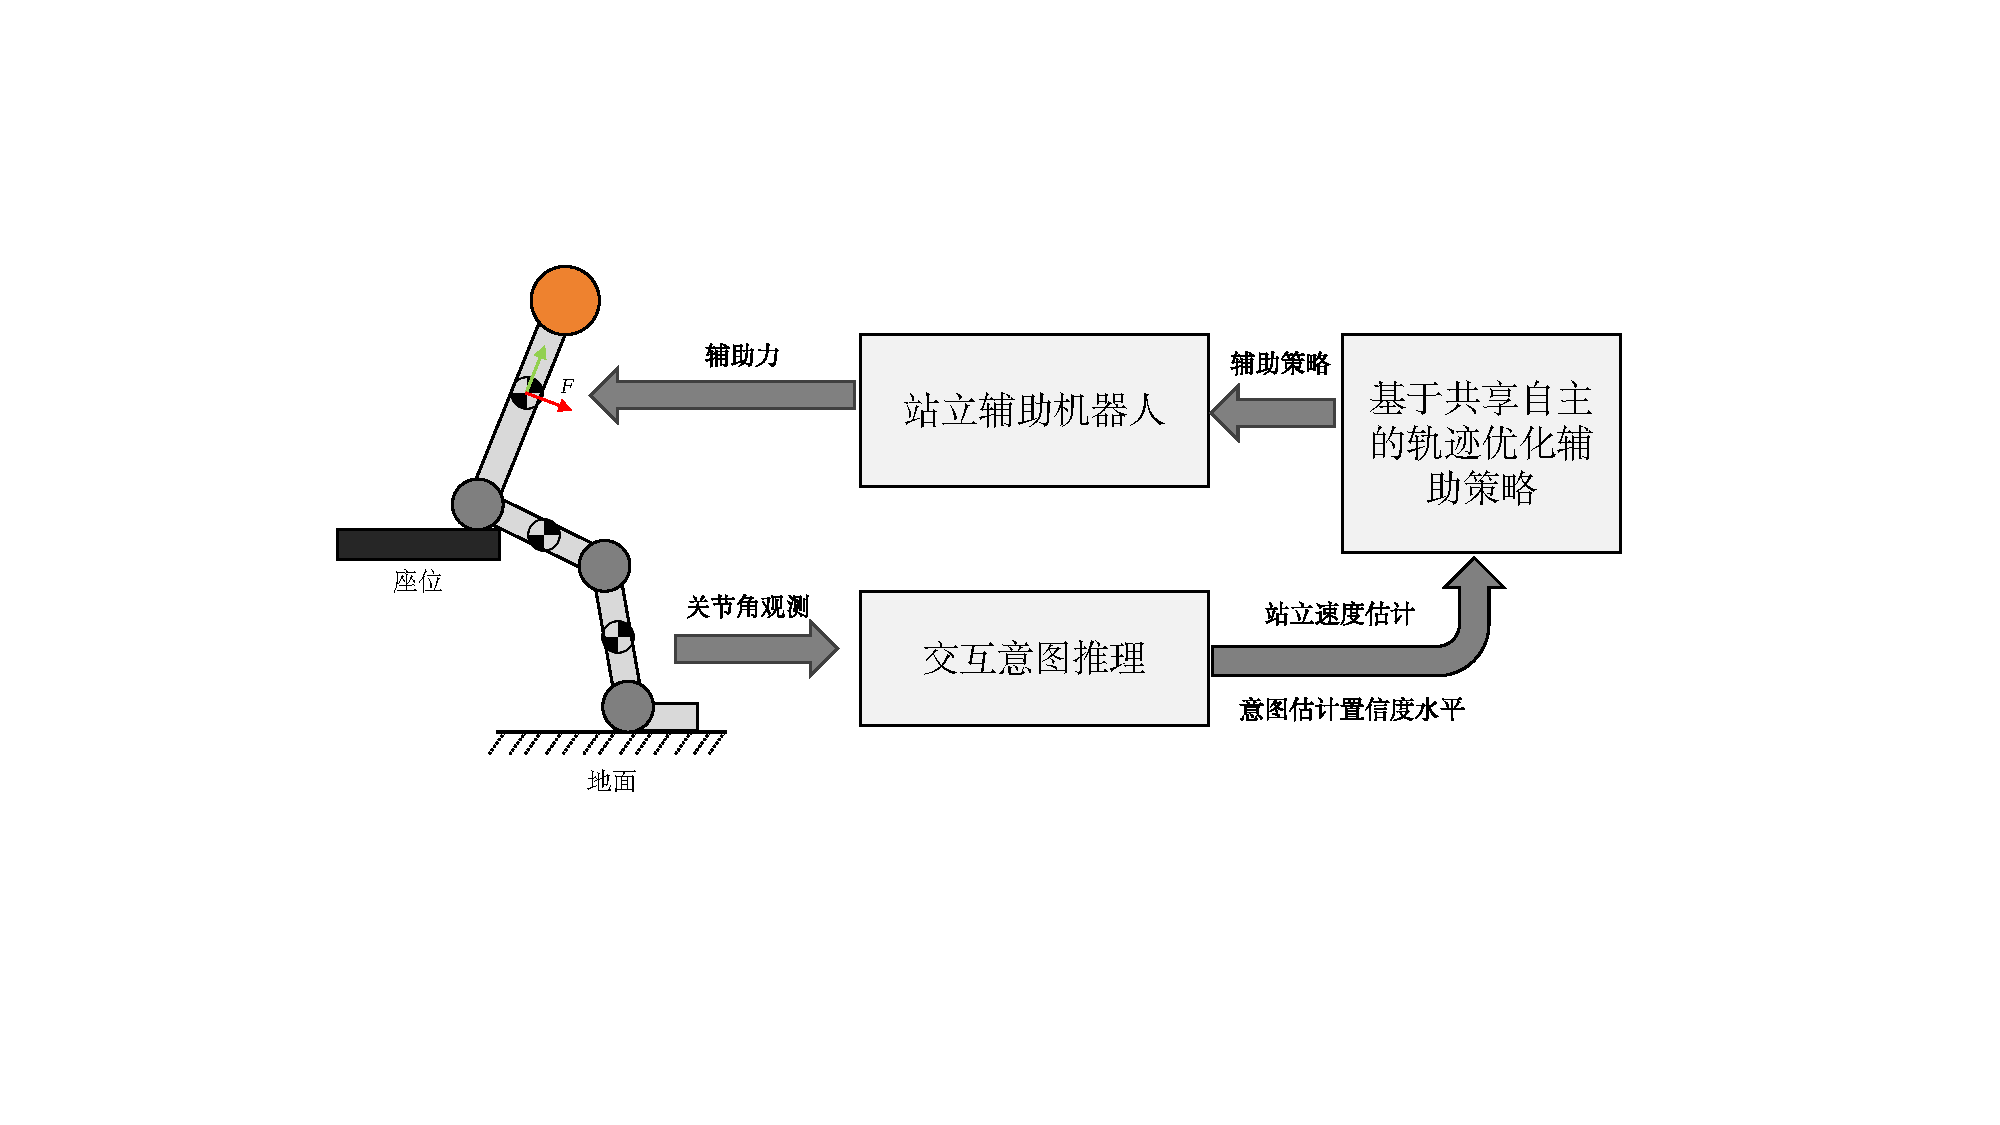
\includegraphics[width=1\textwidth]{figures/4-Fig-2.pdf}
    \caption{基于共享自主的轨迹优化框架结构图}
    \label{fig:4-2}
\end{figure}

\section{概率化的动态运动基元(PDMP)} 
大量的研究使用不同的方法实现人机交互过程中的意图推理,其中目前最为常见的为基于数据驱动模型的方法。该类方法主要通过采集实验数据$\mathbf{D}$构建一个关于意图$I$和当前观测数据$Y$的后验概率模型$P(I|Y,D)$。典型的方法包括基于神经网络的深度学习模型和常见的经典机器学习算法。其中,深度学习模型涵盖循环神经网络(RNN)、长短时记忆网络(LSTM)和Transformer;而经典机器学习算法包括决策树、随机森林、支持向量机(SVM)和逻辑回归等。尽管相关研究在多项任务具有良好的表现,但是在康复辅助机器人的应用开发中,基于数据驱动的方法在难以获取大量人体运动数据的情况下仍然较难实现。此外,由于康复辅助机器人需要保证系统安全性,因此对于相关算法的可解释性也提出了一定要求。

因此,针对STS运动时间预测的这一典型场景,通过考虑人机交互当中的不确定性因素,本小节设计了一种基于随机概率模型匹配的交互意图推理方法。其主要目标为最大化一个关于由时间缩放参数$\tau$控制的交互元模型$M$为先验的似然函数$P(Y,I|M,\tau)$。在意图推理中,通过计算概率模型最大化后验概率进而对用户输入进行分类,以确定其所属的意图类别,并基于迭代优化算法优化参数$\tau$进而确定运动意图。因此,选用合适的模型$M$表征坐立运动对于提高数据利用率至关重要,在本章研究中通过将离散DMP模型改写为一个带有不确定性项的动态系统形式实现了这一目标。由于DMP模型是一种One-Shot学习方法,因此可以仅依靠单条示教数据轨迹实现意图预测,极大地提高了数据利用率。

回顾第二章中在2.3.1节关于DMP模型的介绍,一个标准的离散动态运动基元由以下微分方程定义:
\begin{equation}
    \dot{q}=\tau \alpha\left(\beta(g-y)-q\right)+f(x)
    \label{eq:4-7}
\end{equation}
\begin{equation}
    \dot{y}=\tau q 
    \label{eq:4-8}
\end{equation}
\begin{equation}
    \dot{x}=-\tau \alpha_x x
    \label{eq:4-9}
\end{equation}
一般来说,在将DMP用于机器人轨迹示教时,假设轨迹持续时间$τ$和目标位置$g$是已知的。因此,通过事先给定参数$τ$以及目标$g$,DMP可以通过离线学习的权值向量$w=(w_1,...,w_N)^T$对示教轨迹进行参数化。相反,在本章研究中认为DMP的权重$w$是已知的,而用于在拓扑结构上改变轨迹形状的时间缩放参数$\tau$是未知的。假设我们可以通过离线采集的坐立动作示教轨迹得到一个由权重$w$表示并包含$L$个动态运动基元的技能库:
\begin{equation}
    \mathscr{L}=\left\{\Theta^{(1)}, \ldots, \Theta^{(l)}, \ldots, \Theta^{(L)}\right\}
    \label{eq:4-10}
\end{equation}
其中,$\Theta^{(l)}$代表技能库中的一个运动基元模型。当系统知道来自传感器感知的部分观测$\mathbf{Y}$是属于哪一种运动基元,通过将权重$w$代入DMP微分方程中的强迫项,则系统中仅剩的两个未知量为时间缩放系数$\tau$和轨迹结束目标状态$g$。在本研究中为了简化计算过程,我们默认在STS任务中的下肢三关节在完全站立时到达最终位置$g$,且关节角为0,因此$g$为一个固定的常数不参与优化计算。由于相关研究表明,不同速度下STS动作的轨迹具有相同特征,因此运动时间意图推理的计算问题变为:优化时间缩放系数$\tau$使得缩放后的轨迹与当前的观测数据匹配度最高,即最小化由DMP微分方程组迭代产生的轨迹$P$与观测到的轨迹$Y$之间的距离。

为了实现这一目标,研究基于一个线性动态系统的形式重新改写了DMP模型的系统动力方程,并以时间常数$τ$作为其中的一个关键不确定系统参数。因此,对$τ$的估计就变成了一个系统辨识问题,并通过计算概率$p(Y,P|τ)$度量观测$Y$和模型状态$P$之间的相似性。首先基于欧拉法对一个单自由度离散DMP模型的线性微分方程进行离散化:
\begin{equation}
    \begin{aligned}
    x_t & =-\alpha_x x_{t-1} \tau \Delta t+x_{t-1} \\
    q_t & =\left(\alpha\left(\beta\left(g-p_{t-1}\right)-q_{t-1}\right)+s f\left(x_{t-1}\right)\right) \tau \Delta t+q_{t-1} \\
    p_t & =q_{t-1} \tau \Delta t+p_{t-1}
    \end{aligned}
    \label{eq:4-11}
\end{equation}
假设DMP状态转移以及来自传感器的观测不确定性是服从一个高斯分布的,则可以将以上差分方程写成一个带有高斯噪声项的线性系统。设$z_t = [q_t,p_t]^T$为隐状态变量,$y_t$为在$t$时刻的观测量,$\Delta t$离散积分步长,则一个可以编码单自由度轨迹的概率动态运动基元(PDMP)定义如下:
\begin{equation}
    \begin{aligned}
    & z_t=\mathbf{A}_1 z_{t-1}+\mathbf{A}_2 z_{t-1} \tau+\mathbf{B} * \tau * u_{t-1}+\varepsilon \\
    & y_t=\mathbf{C} z_t+\nu
    \end{aligned}
    \label{eq:4-12}
\end{equation}
其中噪声项$\varepsilon \backsim \mathcal N(0,R)$以及$\nu \backsim \mathcal N(0,Q)$,状态转移矩阵$A_1$和$A_2$分别定义为:
\begin{equation}
    \mathbf{A}_1=\left(\begin{array}{ll}
    1 & 0 \\
    0 & 1
    \end{array}\right), \mathbf{A}_2=\left(\begin{array}{cc}
    -\alpha \Delta t & -\alpha \beta \Delta t \\
    \Delta t & 0
    \end{array}\right)
    \label{eq:4-13}
\end{equation}
输入控制矩阵$\mathbf{B}$和观测矩阵$\mathbf{C}$定义如下:
\begin{equation}
    \mathbf{B}=\left(\begin{array}{c}
    \Delta t \\
    0
    \end{array}\right), \mathbf{C}=\left(\begin{array}{ll}
    0 & 1
    \end{array}\right)
    \label{eq:4-14}
\end{equation}
由强迫项组成的输入量$u_t$为:
\begin{equation}
    u_t=\alpha \beta g+ f\left(x_t\right)
    \label{eq:4-15}
\end{equation}

\section{基于期望最大化算法的人体坐立运动时间预测}
\subsection{期望最大化算法}
期望最大化算法(EM)是一种处理含有隐变量或缺失数据概率模型参数估计的迭代优化算法。它通过交替执行求期望步骤(E步)和最大化步骤(M步)将复杂问题拆解成简单子问题,实现极大似然估计。尽管EM算法的收敛性只能保证找到局部最大值,但它仍被广泛用于处理数据缺失及众多机器学习参数估计问题,例如高斯混合模型和隐马尔可夫模型。其实现步骤如下:

\begin{enumerate}
\item 问题定义:给定观测数据$\mathbf{Y}$和由模型控制的隐变量$\mathbf{Z}$,期望最大化的目标是找到使观测数据出现概率最大的模型参数$θ$,即最大化似然函数$p(\mathbf{Y}|\mathbf{Z}, θ)$。

\item 初始化:随机选择一组初始参数$θ(0)$,作为迭代的起点。

\item E步:在给定当前参数$θ(k)$的情况下,计算隐变量$\mathbf{Z}$的条件概率分布$p(\mathbf{Z}|\mathbf{Y}, θ(k))$。这一步也被称为“求期望”。

\item M步(Maximization-step):使用E步中计算出的条件概率分布$p(\mathbf{Z}|\mathbf{Y}, θ(k))$来最大化Q函数:$Q(θ|θ(k))$ = $\sum p(\mathbf{Z}|\mathbf{Y}, θ(k)) * log(p(\mathbf{Y}, \mathbf{Z}|θ))$。这一步也被称为``求极大''。求解Q函数的导数并令其为0,可以得到新的参数$θ(k+1)$。

\item 收敛判断:检查新参数$θ(k+1)$与当前参数$θ(k)$之间的差异是否小于预设的阈值,或者达到最大迭代次数。如果满足收敛条件,则停止迭代;否则,返回第3步继续迭代。
\end{enumerate}

\subsection{基于EM算法的PDMP模型时间缩放参数优化}
在离线阶段训练获得关于坐立人体运动轨迹表征的权重向量$\mathbf{w}$后,控制PDMP模型生成轨迹的所有参数包括:
\begin{equation}
    \theta_{\text {all }}=\left\{\mathbf{w}, \tau, g, \mathbf{A}_1, \mathbf{A}_2, \mathbf{B}, \mathbf{C}, \mathbf{Q}, \mathbf{R}\right\}
    \label{eq:4-16}
\end{equation}
其中除了时间缩放系数$\tau$是未知的,其余的参数在本任务中都已知。在应用中,当获得关于参与者下肢的关节角度观测$\mathbf{Y}=\{ y_t\}_1^T$后,以及隐状态$\mathbf{Z}=\{z_t\}_1^T$,可以定义联合概率函数:
\begin{equation}
    p(\mathbf{Y}, \mathbf{Z} \mid \tau) = 
    p(\mathbf{Y} \mid  \mathbf{Z}, \tau) \cdot p(\mathbf{Z} \mid  \tau)
    \label{eq:4-17}
\end{equation}
对以上联合概率取对数后,由于通过感知系统无法直接获得关于隐状态$\mathbf{Z}$的观测,因此需要通过对隐状态求取期望消除其随机性,并在最大化步骤中使得优化目标函数Q的值不断增大直到变化速度小于所设定的阈值或达到优化迭代次数上限。最后,可以获得估计参数$\tau$的优化目标函数为:
\begin{equation}
    Q\left(\boldsymbol{\tau}, \boldsymbol{\tau}_{old}\right)=\mathbb{E}_{\mathbf{Z} \mid \tau^{old}}[\ln p(\mathbf{Y}, \mathbf{Z} \mid \tau)]
    \label{eq:4-18}
\end{equation}
其中,$\tau_{old}$为上次迭代得到的历史参数,由于假设了系统不确定性和观测不确定性是服从高斯分布的,且编码动作的PDMP模型是线性的,因此可以得到待辨识参数$\tau$的解析迭代求解方法,其推导过程如下:

在本研究中,离散后的三自由度PDMP模型状态$z_t\in \mathbb{R}^{6}$在每一个时刻都服从以$\mathbf{A_1}z_{t-1}+\mathbf{A_2}z_{t-1}\tau+\mathbf{B}u_{t-1}\tau$为期望,以$\mathbf{R} \in \mathbb{R}^{6\times 6}$为协方差矩阵的多维高斯分布:
\begin{equation}
  z_t \sim \mathcal N(\mathbf{A_1}z_{t-1}+\mathbf{A_2}z_{t-1}\tau+\mathbf{B}u_{t-1}\tau,\mathbf{R})
  \label{eq:4-19}
\end{equation}

设在$T_{obs}$时刻的获得的观测数据为$\mathbf{Y}=\{y_1,y_2,...,y_{T_{obs}}\}$,对应的隐状态为$\mathbf Z = \{z_1,z_2,...,z_{T_{obs}}\}$,对式\ref{eq:4-21}两边同时取对数,当其满足马尔科夫齐次性假设和马尔科夫观测独立性假设时,可以得到以下求和项:
\begin{equation}
    \begin{aligned}
    \ln p(\mathbf{Y}, \mathbf{Z} \mid \tau)= & \sum_{t=1}^T \ln p\left(y_t \mid z_t, \mathbf{C}, \mathbf{R}\right)+\ln p\left(z_1\right) \\
    & +\sum_{t=2}^T \ln p\left(z_t \mid z_{t-1}, \mathbf{A}_1, \mathbf{A}_2, \mathbf{B}, u_{t-1}, \mathbf{Q}, \tau, g\right)
    \end{aligned}
    \label{eq:4-20}
\end{equation}
其中式中第一个求和项为状态观测项,第二项为常数,第三项为状态转移概率求和项。由于存在隐变量$z_t$,基于旧的时间缩放系数$\tau_{old}$对隐状态求期望,代入式\ref{eq:4-18}中的优化目标函数$ Q\left(\tau, \tau^{old}\right)$函数并展开:
\begin{equation}
\begin{aligned}
    Q\left(\tau, \tau^{old}\right)
    &=\mathbb{E}_{z \mid \tau^{old}}\left[\ln p(\mathbf{Y}, \mathbf{Z} \mid \tau)\right]\\
    & =\mathbb{E}_{z \mid \tau^{old}}\left[\sum_{t=1}^T \ln p\left(y_t \mid z_t, \tau\right)+\ln p\left(z_1\right)+\sum_{t=2}^T \ln p\left(z_t \mid z_{t-1}, \tau\right)\right] \\
    & =\mathbb{E}_{z \mid \tau^{old}}\left[\sum_{t=2}^T \ln p\left(z_t \mid z_{t-1}, \tau\right)\right] + \eta 
\end{aligned}
\label{eq:4-21}
\end{equation}
其中$\eta=\mathbb{E}_{z \mid \tau^{old}} \left[\sum_{t=1}^T \ln p\left(y_t \mid z_t, \tau\right) + \ln p\left(z_1\right)\right]$为一个与隐状态变量$z$无关的常数。根据之前对于PDMP系统的状态转移的假设,状态转移概率服从一个多维高斯分布,因此关于状态转移条件概率的概率密度函数表达式为:
\begin{equation}
    p\left(z_t \mid z_{t-1}, \tau\right)=\frac{1}{(2 \pi)^{\frac{n}{2}}|\mathbf{R}|^{\frac{1}{2}}} \cdot e^{-\frac{1}{2}\left[\left(z_t-\mu\right)^T \mathbf{R}^{-1}\left(z_t-\mu\right)\right]}
    \label{eq:4-22}
\end{equation}
其中$n=6$,为多维高斯分布的维度,在本研究中等于观测的关节角度数量的二倍,将上式取对数后:
\begin{equation}
    \ln p\left(z_t \mid z_{t-1}, \tau\right)=-\pi^{-\frac{n}{2}}\ln\mathbf{|R|}-\frac{1}{2}\left[\left(z_t-\mu\right)^T \mathbf{R}^{-1}\left(z_t-\mu\right)\right]
    \label{eq:4-23}
\end{equation}
则迭代优化目标函数为:
\begin{equation}
    Q\left(\tau, \tau^{old}\right)
    =\mathbb{E}_{z \mid \tau^{old}}\left[\sum_{t=2}^T-\pi^{-\frac{n}{2}}\ln\mathbf{|R|}-\frac{1}{2}\left(z_t-\mu\right)^T \mathbf{R}^{-1}\left(z_t-\mu\right)\right] + \eta
    \label{eq:4-24}
\end{equation}
对上式求关于时间缩放系数$\tau$的导数,首先使用迹技巧求优化目标函数的微分:
\begin{equation}
    d Q=\operatorname{tr}\left(\frac{\partial Q^T}{\partial \mu} \cdot d \mu\right)
    \label{eq:4-25}
\end{equation}
将\ref{eq:4-24}代入上式得到:
\begin{equation}
    \begin{aligned}
    d Q\left(\tau, \tau^{old}\right)
    & =\operatorname{tr}\left[\mathbb{E}_{z \mid \tau^{old}}\left[\sum_{t=2}^T-\frac{1}{2} \cdot 2 \left(\mathbf{R}^{-1}\left(z_t-\mu\right)\right)^T \cdot d \mu\right]\right] \\
    & =\mathbb{E}_{z \mid \tau^{old}}\left[\operatorname{tr}\left[\sum_{t=2}^T-\left(z_t-\mu\right)^T \left(\mathbf{R}^{-1}\right)^T \cdot d \mu\right]\right] \\
    & =\mathbb{E}_{z \mid \tau^{old}}\left[\operatorname{tr}\left[\sum_{t=2}^T-\left(z_t-\mu\right)^T \left(\mathbf{R}^{-1}\right)^T \cdot d\left(\mathbf{A_1} z_{t-1}+\mathbf{A_2} z_{t-1} \tau+\mathbf{B} u_{t-1} \tau\right)\right]\right] \\
    & =\mathbb{E}_{z \mid \tau^{old}}\left[\operatorname{tr}\left[\sum_{t=2}^T-\left(z_t-\mu\right)^T \left(\mathbf{R}^{-1}\right)^T\left(\mathbf{A_2}z_{t-1} d \tau+\mathbf{B} u_{t-1} d \tau\right)\right]\right] \\
    & =\mathbb{E}_{z \mid \tau^{old}}\left[\operatorname{tr}\left[\sum_{t=2}^T-\left(z_t-\mu\right)^T \left(\mathbf{R}^{-1}\right)^T(\mathbf{A_2} z_{t-1}+\mathbf{B} u_{t-1}) d \tau \right]\right]
    \end{aligned}
    \label{eq:4-26}
\end{equation}
则优化目标函数$Q$关于时间缩放系数$\tau$的导数为:
\begin{equation}
    \frac{d Q}{d \tau}=\mathbb{E}_{z \mid \tau^{old}}\left[\sum_{t=2}^T -\left(z_t-\mu\right)\left(\mathbf{A_2} z_{t-1}+\mathbf{B} u_{t-1}\right)^T\mathbf{R}^{-1}\right]
    \label{eq:4-27}
\end{equation}
令上式的导数为0:
\begin{equation}
    \mathbb{E}_{z \mid \tau^{old}}\left[\sum_{t=2}^T -\left(z_t-\mu\right)\left(\mathbf{A_2} z_{t-1}+\mathbf{B} u_{t-1}\right)^T\mathbf{R}^{-1}\right] = 0
    \label{eq:4-28}
\end{equation}
由于协方差矩阵$\mathbf{R}$为实对称矩阵,则:
\begin{equation}
    \mathbb{E}_{z \mid \tau^{old}}\left[\sum_{t=2}^T \left(z_t-\mu\right)\left(z_{t-1}^T\mathbf{A_2}^T +u_{t-1}^T\mathbf{B}^T \right)\right] = 0
    \label{eq:4-29}
\end{equation}
将式\ref{eq:4-19}中的期望代入上式$\mu$:
\begin{equation}
    \mathbb{E}_{z \mid \tau^{old}}\left[\sum_{t=2}^T \left(z_t-\mathbf{A_1}z_{t-1}-\mathbf{A_2}z_{t-1}\tau-\mathbf{B}u_{t-1}\tau \right)\left(z_{t-1}^T\mathbf{A_2}^T +u_{t-1}^T\mathbf{B}^T \right)\right] = 0
    \label{eq:4-30}
\end{equation}
展开上式:
\begin{equation}
    \begin{gathered}
    \sum_{t=2}^T \mathbb{E}_{z \mid \tau^{old}}\left[z_tz_{t-1}^T\mathbf{A_2}^T + z_tu_{t-1}^T\mathbf{B}^T -\mathbf{A_1}z_{t-1}z_{t-1}^T\mathbf{A_2}^T - \mathbf{A_1}z_{t-1}u_{t-1}^T\mathbf{B}^T \right. \\ 
    \left. - \mathbf{A_2}z_{t-1}z_{t-1}^T\mathbf{A_2}^T\tau -\mathbf{A_2}z_{t-1}u_{t-1}^T\mathbf{B}^T\tau - \mathbf{B}u_{t-1}z_{t-1}^T\mathbf{A_2}^T\tau - \mathbf{B}u_{t-1}u_{t-1}^T\mathbf{B}^T\tau\right] = 0
    \end{gathered}
    \label{eq:4-31}
\end{equation}

\begin{algorithm}[htb]
    \SetAlgoLined
    \KwData{DMP的权重向量$w$,$\tau$的初始值,参数$\mathbf{A_1}$,$\mathbf{A_2}$,$\mathbf{B}$,$\mathbf{C}$,协方差矩阵$\mathbf{R}$和$\mathbf{Q}$}
    \KwIn{基于运动捕捉系统对人体关节运动的观测$\mathbf{Y}_{1:T_{obs}}$}

    \KwResult{基于当前部分观测数据对于参数$\tau$的估计,似然概率$l_{T_{obs}}=\sum_{t=1}^{T_{obs}} \text{ln}c_t$}
  
    \For{i=1:Epoch}{
      给定初值$
      \hat{z}_{f, 0}^{+}=\mathbb{E}\left[z_0\right]$和$\mathbf{V}_{f, 0}=\mathbb{E}\left[\left(z_0-\hat{z}_{f, 0}^{+}\right)\left(z_0-\hat{z}_{f, 0}^{+}\right)^T\right]
      $\;
      进行前向卡尔曼滤波迭代计算\;
      \For{t=1:$T_{obs}$}
      {
        $\begin{aligned}
            &\mathbf{P}_{f, t}=\mathbf{A} \mathbf{V}_{f, t-1} \mathbf{A}+\mathbf{Q} \\
            &\mathbf{K}=\mathbf{P}_{f, t} \mathbf{C}^T\left(\mathbf{C P}_{f, t} \mathbf{C}^T+\mathbf{R}\right)^{-1} \\
            &\hat{z}_{f, t}^{-}=\mathbf{A} \hat{z}_{f, t-1}^{+}+\mathbf{B} u_{t-1} \\
            & \hat{z}_{f, t}^{+}=\hat{z}_{f, t}^{-}+\mathbf{K}\left(y_t-\mathbf{C} \hat{z}_{f, t}^{-}\right) \\
            &\mathbf{V}_{f, t}=(\mathbf{I}-\mathbf{K} \mathbf{C}) \mathbf{P}_{f, t} \\
            &c_t=\mathscr{N}\left(y_t \mid \mathbf{C} \hat{z}_{f t}^{-}, \mathbf{C} \mathbf{P}_{f, t} \mathbf{C}^T+\mathbf{R}\right) \\
            &l_t= \text{ln}c_t + l_{t-1}
        \end{aligned}$
      }{
        进行反向卡尔曼平滑计算必要的期望项\;
        \For{t=$T_{obs}-1$:1}
        {
            $\begin{aligned} & \mathbf{J}_t=\mathbf{V}_{f, t} \mathbf{A}\left(\mathbf{P}_{f, t+1}\right)^{-1} \\ & \mathbf{V}_t=\mathbf{V}_{f, t}-\mathbf{J}_t\left(\mathbf{P}_{f, t+1}-\mathbf{V}_{t+1}\right) \mathbf{J}_t^T \\ & \hat{z}_t=\hat{z}_{f, t}^{+}+\mathbf{J}_t\left(\hat{z}_{t+1}-\hat{z}_{f, t+1}^{-}\right) \\ & \mathbb{E}\left[z_t\right]=\hat{z}_t \\ & \mathbb{E}\left[z_t z_t^T\right]=\mathbf{V}_t+\hat{z}_t \hat{z}_t^T \\ & \mathbb{E}\left[z_t z_{t-1}^T\right]=\mathbf{J}_{t-1} \mathbf{V}_t+\hat{z}_t \hat{z}_{t-1}\end{aligned}$
        }
        \For{t=2:$T_{obs}$}
        {
            $\begin{gathered}\Sigma_1=\sum_{t=2}^T \operatorname{tr}\left(\mathbb{E}\left[z_t z_{t-1}^T\right] \mathbf{A}_2^T\right)+\operatorname{tr}\left(\mathbb{E}\left[z_t\right] u_{t-1}^T \mathbf{B}^T\right)- \operatorname{tr}\left(\mathbb{E}\left[z_{t-1} z_{t-1}^T\right] \mathbf{A}_1 \mathbf{A}_2^T\right) \\ - \operatorname{tr}\left(\mathbb{E}\left[z_{t-1}\right] \mathbf{A}_1 u_{t-1}^T \mathbf{B}^T\right)\end{gathered}$

            $\Sigma_2=\sum_{t=2}^T \operatorname{tr}\left(\mathbb{E}\left[z_{t-1} z_{t-1}^T\right] \mathbf{A}_2 \mathbf{A}_2{ }^T\right)+2 \operatorname{tr}\left(\mathbf{B} u_{t-1} \mathbb{E}\left[z_{t-1}^T\right] \mathbf{A}_2{ }^T\right)+\operatorname{tr}\left(\mathbf{B} u_{t-1} u_{t-1}^T \mathbf{B}^T\right)$
        }
        $\tau=\Sigma_1 / \Sigma_2$ \;
      }
    }
    \caption{基于EM的PDMP轨迹时间缩放参数优化}
    \label{algo:4-1}
\end{algorithm}
整理可得:
\begin{equation}
    \begin{gathered}
    \sum_{t=2}^T \mathbb{E}_{z \mid \tau^{old}}\left[z_tz_{t-1}^T\mathbf{A_2}^T + z_tu_{t-1}^T\mathbf{B}^T -\mathbf{A_1}z_{t-1}z_{t-1}^T\mathbf{A_2}^T - \mathbf{A_1}z_{t-1}u_{t-1}^T\mathbf{B}^T\right] = \\ 
    \sum_{t=2}^T \mathbb{E}_{z \mid \tau^{old}}\left[\mathbf{A_2}z_{t-1}z_{t-1}^T\mathbf{A_2}^T\tau +\mathbf{A_2}z_{t-1}u_{t-1}^T\mathbf{B}^T\tau + \mathbf{B}u_{t-1}z_{t-1}^T\mathbf{A_2}^T\tau +\mathbf{B}u_{t-1}u_{t-1}^T\mathbf{B}^T\tau\right]
    \end{gathered}
    \label{eq:4-32}
\end{equation}
对等式两边同时取迹,等式保持不变,可以得到$\tau$更新的解析表达式:
\begin{equation}
    \tau^{new} = \frac{\Sigma_1}{\Sigma_2}
    \label{eq:4-33}
\end{equation}
其中:
\begin{equation}
    \begin{gathered}
    \Sigma_1  = \sum_{t=2}^T \operatorname{tr}\left(\mathbb{E}\left[z_tz_{t-1}^T\right]\mathbf{A_2}^T\right) + \operatorname{tr}\left(\mathbb{E}\left[z_t\right]u_{t-1}^T\mathbf{B}^T\right) \\- \operatorname{tr}\left(\mathbb{E}\left[z_{t-1}z_{t-1}^T\right]\mathbf{A_1}\mathbf{A_2}^T\right) - \operatorname{tr}\left(\mathbb{E}\left[z_{t-1}\right]\mathbf{A_1}u_{t-1}^T\mathbf{B}^T\right) \\
    \end{gathered}
    \label{eq:4-34}
\end{equation}
\begin{equation}
    \Sigma_2  = \sum_{t=2}^T \operatorname{tr}\left(\mathbb{E}\left[z_{t-1}z_{t-1}^T\right]\mathbf{A_2}\mathbf{A_2}^T\right) + 2 \operatorname{tr}\left(\mathbf{B}u_{t-1}\mathbb{E}\left[z_{t-1}^T\right]\mathbf{A_2}^T\right) +\operatorname{tr}\left(\mathbf{B}u_{t-1}u_{t-1}^T\mathbf{B}^T\right)
    \label{eq:4-35}
\end{equation}

在$\tau$的迭代更新公式中,有三个期望是未知的,可以使用卡尔曼平滑方法进行计算\cite{bishopPatternRecognitionMachine2006},其计算方法如下:
\begin{equation}
    \begin{aligned}
    \mathbb{E}\left[z_{t-1}\right] & =\hat{z}_{t-1} \\
    \mathbb{E}\left[z_{t-1} z_{t-1}^T\right] & =\operatorname{cov}\left(z_{t-1}, z_{t-1}\right)+\hat{z}_{t-1} \hat{z}_{t-1}^T \\
    \mathbb{E}\left[z_t z_{t-1}^T\right] & =\operatorname{cov}\left(z_t, z_{t-1}\right)+\hat{z}_t \hat{z}_{t-1}^T .
    \end{aligned}
    \label{eq:4-36}
\end{equation}
其中的协方差矩阵可由卡尔曼滤波得到,基于EM的PDMP轨迹时间缩放参数优化算法的完整流程如算法\ref{algo:4-1}所示。

\subsection{基于先验知识库的人体坐立运动时间意图估计}
由于EM算法需要给定参数$\tau$的初值,而参数的初值选择直接影响EM算法的迭代收敛效率以及能否得到全局最优解,导致其在运动时间估计中无法适应大范围的时间变化。因此在实验中分别离线采集了慢速、中等速度、快速三种坐立动作轨迹,并基于此通过PDMP模型构建了运动先验知识库$\mathscr{L}$。

\begin{figure}[htb]
    \centering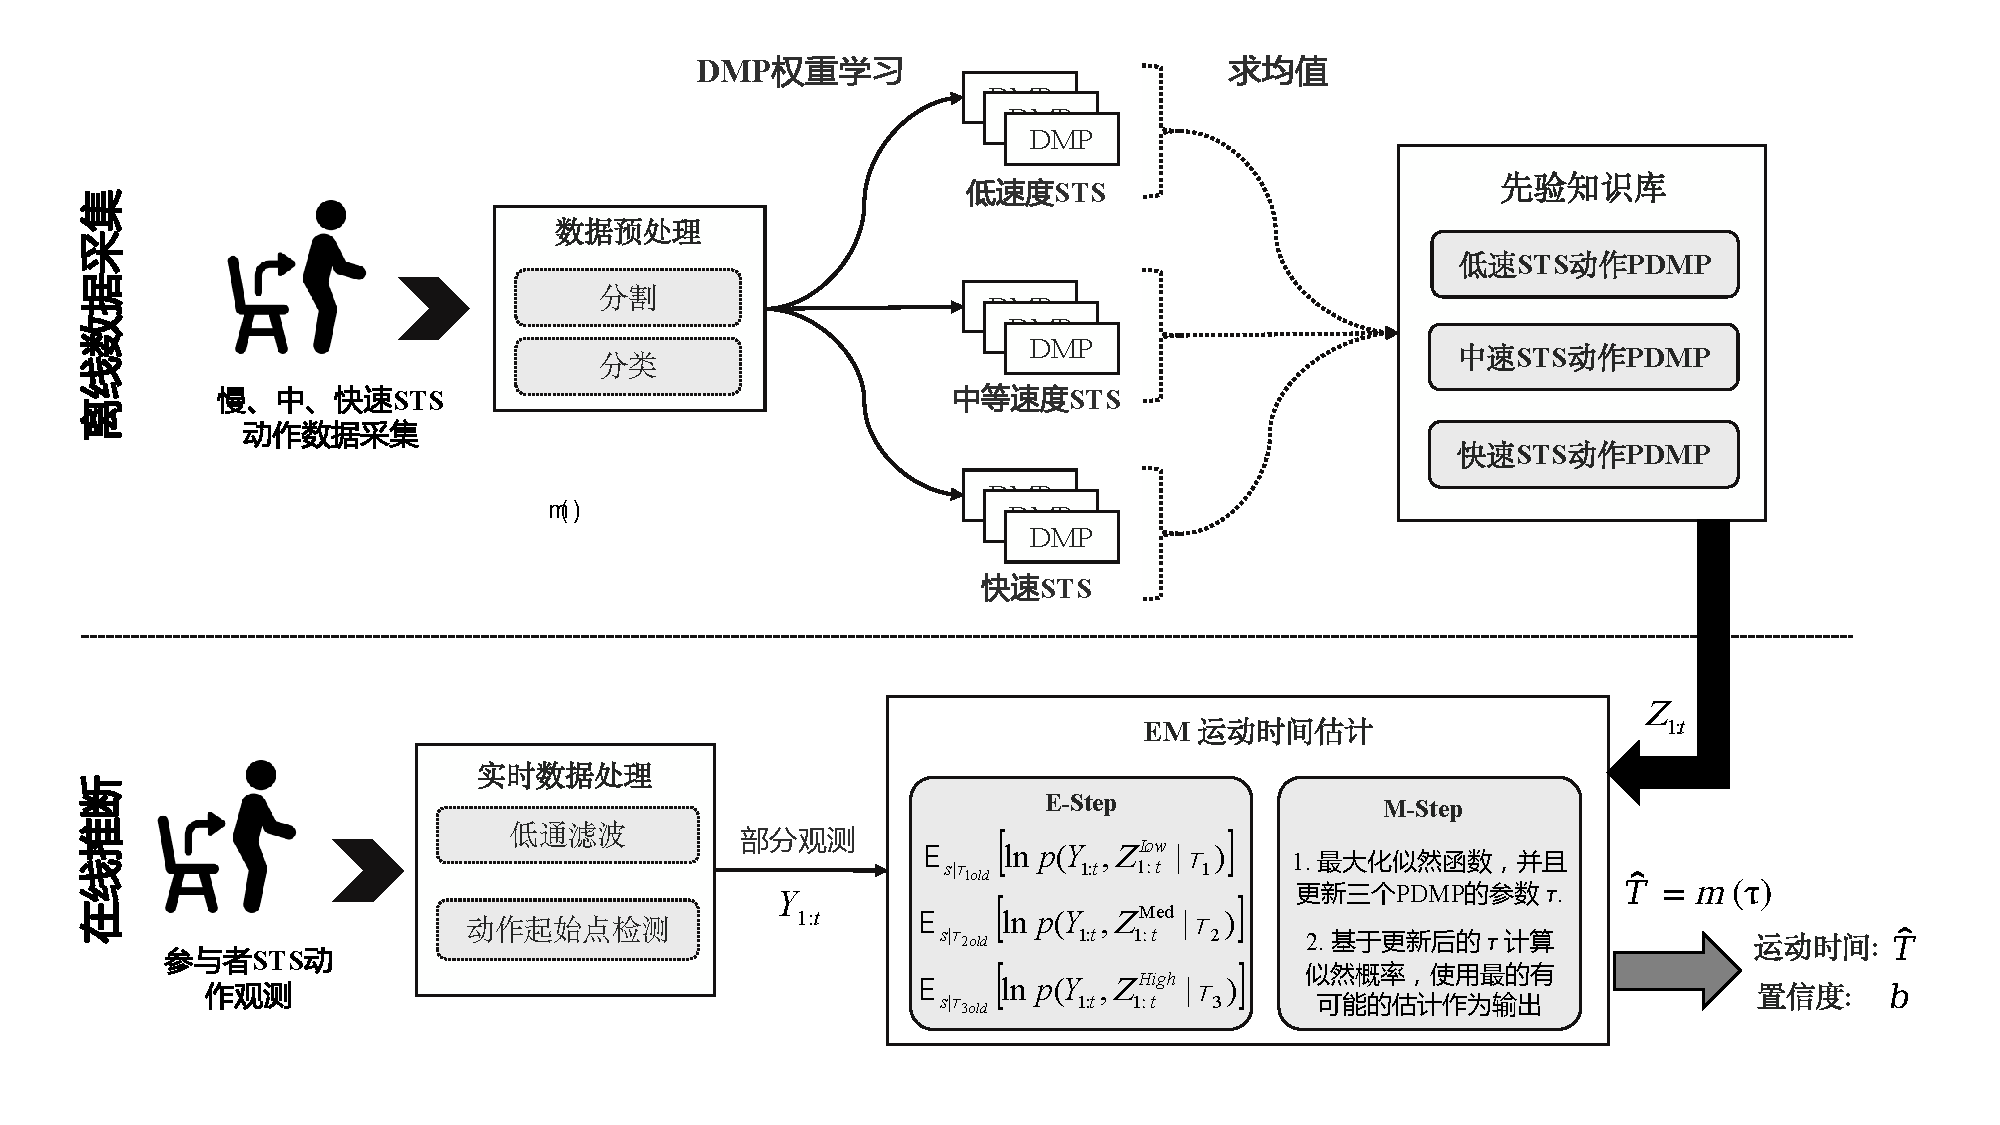
\includegraphics[width=1\textwidth]{figures/4-Fig-3.pdf}
    \caption{人体坐立运动时间估计方法结构图}
    \label{fig:4-3}
\end{figure}

\begin{equation}
    \mathscr{L}=\left\{\Theta^{low}, \Theta^{medium}, \Theta^{high}\right\}
    \label{eq:4-37}
\end{equation}
其中每个由$\Theta$表示的PDMP模型由其各自不同的参数集合参数化,在观测到被辅助对象下肢运动姿态后,选择匹配度最好的模型的预测结果作为STS运动时间意图推断的结果。库中第$m$个运动基元可通过以下的参数化形式表示:
\begin{equation}
    \Theta ^{m}=\left\{\mathbf{w}^{m}, \tau^{m}, g, \mathbf{A}_1, \mathbf{A}_2, \mathbf{B}, \mathbf{C}, \mathbf{Q}^{m}, \mathbf{R}^{m}\right\}
    \label{eq:4-38}
\end{equation}
当通过离线示教获得坐立运动先验知识库$\mathscr{L}$后,可以通过算法\ref{algo:4-1}中的卡尔曼前向滤波中关于似然函数的积分值$l_{obs}$实现在线的模板匹配识别。当在每个时间步得到新的关于人体运动的观测数据后,所提出方法并行地将当前所有观测到的运动轨迹与$\mathscr{L}$中的每个运动基元进行匹配,并且对于每个PDMP模型迭代优化时间缩放系数$\tau^{m}$用于估计该运动在当前先验模型下在何时结束。估计是通过周期性地执行在对于观测$\mathbf{Y}_{1:t}$的EM算法来实现的,直到所有完成坐立运动的数据都被观察到,或当观测与某一个运动基元的相关性超过了所设定的阈值。
\begin{algorithm}[htb]
    \SetAlgoLined
    \KwData{先验STS运动技能库$\mathscr{L}$}
    \KwIn{基于运动捕捉系统对人体关节运动的观测$\mathbf{Y}_{1:T_{obs}}$}
    \KwResult{基于当前部分观测数据对于STS运动时间的估计$\hat T$,置信度$b$}
    \For{每获取10个时间步的数据$y_{{(T_{obs}-10)}:T_{obs}}$}
    {
        将$y_{{(T_{obs}-10)}:T_{obs}}$添加到观测序列数据$Y_{1:T_{obs}}$中 \;
        \For{$\Theta ^{m}$ in $\mathscr{L}$}
        {
            基于当前观测$Y_{1:T_{obs}}$,迭代执行EM算法10次优化时间缩放系数$\tau^m$,并记录每次迭代更新后的值$[\tau_m^1,\tau_m^1,...,\tau_m^{10}]$\;
            计算似然函数求和$l_{T_{obs}}^m=\text{ln}p(\mathbf{Y}_{1:T_{obs}}|\Theta ^{m})=\sum_{1}^{T_{obs}} \text{ln}p(y_t|\Theta ^{m})$ \;
        }
        计算先验库中匹配度最高的PDMP模型:$m=argmax_m l_{T_{obs}}^m$\;
        计算坐立运动时间估计值:$\hat T = f_m(\tau_m)$\;
        计算EM迭代过程中参数$\tau$的方差作为估计置信度水平量化指标:$b = 1 - var([\tau_m^1,\tau_m^1,...,\tau_m^{10}]) * 100$\;
    }
    \caption{基于先验模板库的人体坐立运动时间意图估计}
    \label{algo:4-2}
\end{algorithm}

为了减少计算负担,在使用EM优化时间缩放系数$\tau^{m}$时,该方法在实际应用中每累积10个时间步的数据后更新一次观测。在每次更新观测数据后,基于当前观测迭代执行10次EM算法用于优化时间缩放系数$\tau$。迭代完成后,使用匹配度最高的时间缩放系数并经过一个线性映射用于估计完成STS的时间$\hat T=f_m(\tau_m)$。其中映射函数$f_m(\tau^m)$为一个线性函数,用于将无物理意义的时间缩放系数映射到真实的时间。此外,由于EM算法收敛时,迭代过程的参数变化范围会逐步缩小直至收敛,算法在每次更新数据后记录了EM迭代优化参数$\tau$的历史数据,并通过计算迭代数据方差用于量化当前估计的置信度水平$b$,进而实现对共享自主系统中的仲裁函数的调节。关于每个PDMP先验模型的参数优化是独立且并行进行的,其计算时间复杂度以及空间复杂度为线性阶$O(N)$,完整的算法流程在算法\ref{algo:4-2}中给出。

\section{实验与分析}
\subsection{实验环境设置} 
在本研究中,实验招募了三名参与者(平均身高175±5厘米,体重75±10公斤)参与实验。实验环境配备了一套由OptiTrack公司生产的高精度光学动作捕捉系统。实验中我们设置了一个高度为50厘米的座椅,并在其下方放置了一块由AMTI公司制造的测力板,用以精确检测参与者的起身事件。根据光学运动捕捉系统中的Helen Hayes反光标记点放置标准,每位参与者的下肢佩戴了19个反光标记物,用于追踪他们的下肢关节角运动轨迹。实验要求参与者保持静态坐姿,然后分别以快速、中等和缓慢三种速度完成站立-坐下动作,每种速度重复10次。其中参与者被要求在处于站立状态后和完成坐下后都保持1秒钟的静止,用于后期数据分割。为了保证计算的关节运动轨迹符合生物运动学特征,将由运动捕捉记录采集的光学标记点位置数据使用Opensim生物动力/运动学仿真软件计算参与者下肢三个关节在矢状面的关节角度变化曲线。

\subsection{基于三自由度PDMP的坐立动作模型表征} 
上一节基于三连杆模型对人体完成坐立动作的过程进行了分析。在本小节中,通过简化的模型,使用PDMP模型对下肢踝关节、膝关节以及髋关节的运动轨迹进行了编码表征处理。其中,由于数据采集是连续进行的,因此需要对采集得到的轨迹进行分割处理。其中完成坐立运动过程的有效关节运动轨迹是通过计算髋关节$\theta_3$运动的一阶导数$\dot\theta_3$,并在$\dot\theta_3=0$处作为轨迹的分割点实现的。在进行轨迹分割后,仅使用由坐到站的轨迹用于构建先验知识库。为了避免数值积分问题,关节角轨迹使用各个关节的主动活动度参数进行归一化处理。关于关节角度轨迹$X$的归一化关节运动轨迹$X_{norm}$定义为:
\begin{equation}
    X_{norm} = \frac{X-AROM_{min}}{AROM_{max}-AROM_{min}}
    \label{eq:4-39}
\end{equation}
其中$AROM_{min}$和$AROM_{max}$分别代表了下肢关节主动活动度的最小和最大值。设踝关节、膝关节、髋关节在坐立运动过程中的归一化轨迹分别为$X_{1,2,...,10}^{ankle}$、$X_{1,2,...,10}^{knee}$、$X_{1,2,...,10}^{hip}$,使用2.3.3节所述的DMP离线学习方法分别学习各个关节每段坐立运动轨迹,其中基函数的数量设置为$N=20$,起始点设置为归一化关节轨迹的第一个值$p_0=X_i(0)$,轨迹目标$g=[0,0,0]^T$。如图\ref{fig:4-3}所示,在离线阶段基于踝、膝、髋三个关节的归一化运动数据对不同运动速度下的坐立运动进行了建模表征,并将由模型产生的权重向量的均值作为运动先验知识存放在库中。在实验中,我们要求参与者分别按照慢速(完成STS动作约2.5秒)、中等速度(完成STS动作约5秒)、快速三种STS(完成STS动作约7.5秒)进行STS运动10次并采集数据。最终获得了30组有效的STS动作关节运动轨迹片段,构建了基于三种STS速度的PDMP运动先验知识库$\mathscr{L}$。

为了保持同步,三个关节的轨迹由同一个相位变量$x$控制,包含了三个关节轨迹信息的三自由度PDMP的隐变量为$z_t=[z_1,z_2,z_3,p_1,p_2,p_3]^T$分别代表了各个关节独立的DMP隐变量。则系统状态转移矩阵为:
\begin{equation}
    \mathbf{A}_1=\left(\begin{array}{llllll}
    1 & 0 & 0 & 0 & 0 & 0\\
    0 & 1 & 0 & 0 & 0 & 0\\
    0 & 0 & 1 & 0 & 0 & 0\\
    0 & 0 & 0 & 1 & 0 & 0\\
    0 & 0 & 0 & 0 & 1 & 0\\
    0 & 0 & 0 & 0 & 0 & 1
    \end{array}\right)
    \label{eq:4-40}
\end{equation}
\begin{equation}
    \mathbf{A}_2=\left(\begin{array}{cccccc}
    -\alpha_z \Delta t & 0 & 0 & -\alpha_z \beta_z \Delta t & 0 & 0 \\
    0 &-\alpha_z \Delta t & 0 & 0 &-\alpha_z \beta_z \Delta t & 0 \\
    0 & 0 & -\alpha_z \Delta t & 0 & 0 &  -\alpha_z \beta_z \Delta t \\
    \Delta t & 0 & 0 & 0 & 0 & 0 \\
    0 & \Delta t & 0 & 0 & 0 & 0 \\
    0 & 0 & \Delta t &  0 & 0 & 0 \\
    \end{array}\right)
    \label{eq:4-41}
\end{equation}
3自由度DMP的输入控制矩阵$\mathbf{B}$和观测矩阵$\mathbf{C}$定义如下:
\begin{equation}
    \mathbf{B}=\left(\begin{array}{cccccc}
    \Delta t & 0 & 0 & 0& 0& 0\\
    0 & \Delta t & 0 & 0& 0& 0\\
    0 & 0 & \Delta t & 0& 0& 0\\
    0 & 0 & 0 & 0& 0& 0\\
    0 & 0 & 0 & 0& 0& 0\\
    0 & 0 & 0 & 0& 0& 0\\
    \end{array}\right), \mathbf{C}=\left(\begin{array}{llllll}
    0 & 0 & 0 & 1 & 0 &0\\
    0 & 0 & 0 & 0 & 1 &0\\
    0 & 0 & 0 & 0 & 0 &1
    \end{array}\right)
    \label{eq:4-42}
\end{equation}
由强迫项组成的输入量$u_t$为:
\begin{equation}
    u_t=\left(\begin{array}{l}
        \alpha_z \beta_z g+ f\left(x_t\right)_{ankle}\\
        \alpha_z \beta_z g+ f\left(x_t\right)_{knee}\\
        \alpha_z \beta_z g+ f\left(x_t\right)_{hip}
    \end{array}\right)
    \label{eq:4-43}
\end{equation}
其中强迫项由各关节的DMP权重调节,此外观测噪声协方差矩阵和状态转移噪声协方差矩阵$Q\in \mathbf{R}^{6 \times 6}$,$R\in \mathbf{R}^{6 \times 6}$,其可以通过经验设定或通过EM算法迭代更新\cite{bishopPatternRecognitionMachine2006}。

\subsection{实验结果} 
在建立包含了三种运动速度的先验坐立动作知识库后,基于对三位参与者随机站立运动的关节轨迹观测数据,测试了所提出算法的性能表现。我们要求参与者按照随机的站立速度完成站立动作10次,并构建了一个包含30组运动轨迹验证运动数据集用于测试算法。如图\ref{eq:4-3}所示,意图推理是在线进行的,在实验验证中,通过将采集的验证运动数据集迭代更新到所提出坐立运动时间意图推断框架中,模拟测试了算法的在线计算表现。
\begin{figure}[htb]
    \centering\includegraphics[width=1\textwidth]{figures/4-Fig-4.pdf}
    \caption{由$t=1$到$t=6$时刻的坐立实验过程}
    \label{fig:4-4}
\end{figure}

\begin{figure}[!t]
    \centering
    \rotatebox[origin=c]{-90}
    {
        \begin{minipage}{9.5in}
            \centering
            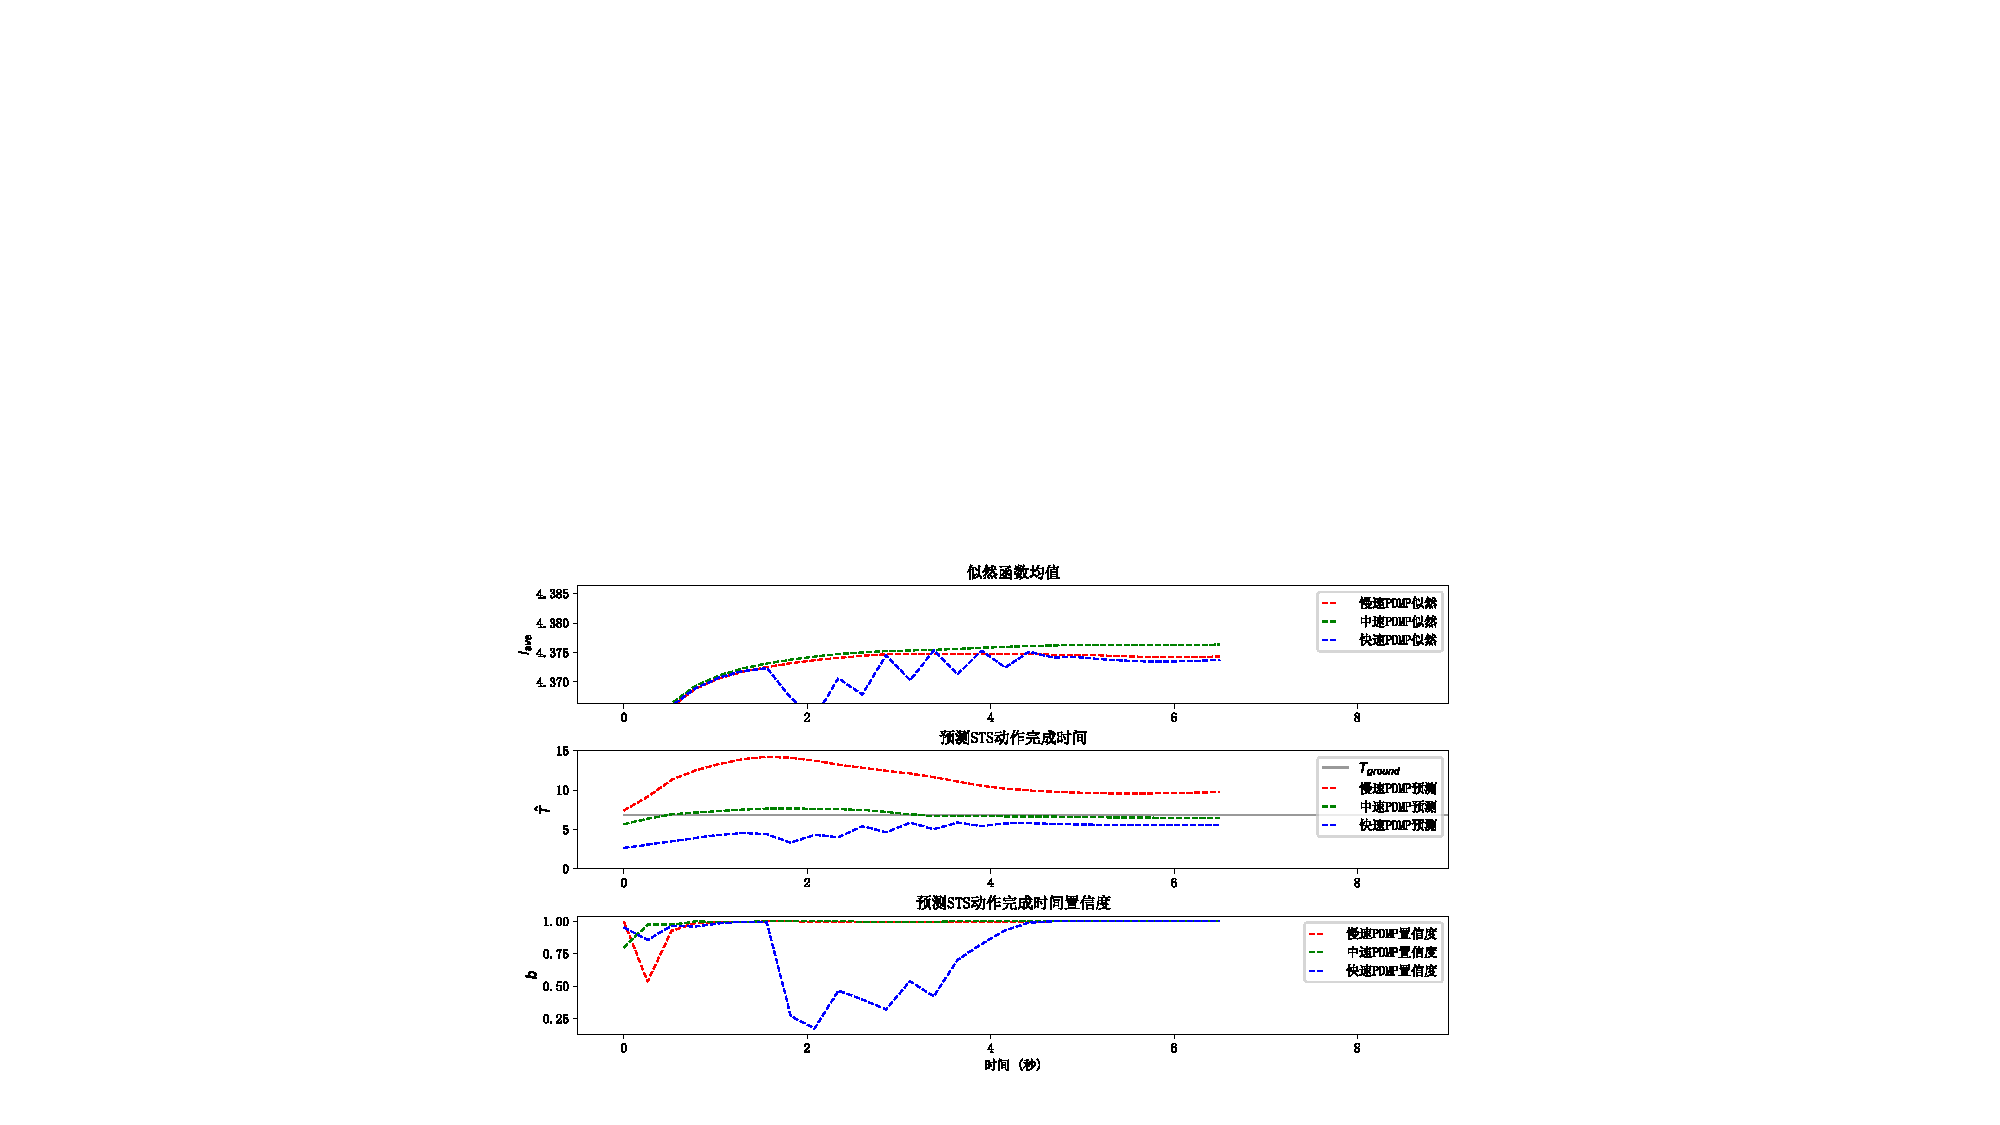
\includegraphics[width=\textwidth]{figures/4-Fig-5.pdf}
            \caption{下肢三关节矢状面运动观测轨迹与模板匹配的轨迹随时间变化的情况}
        \label{fig:4-5}
        \end{minipage}
    }
\end{figure}

在图\ref{fig:4-4}中展示了研究中所进行的坐立实验过程,并在图\ref{fig:4-5}中给出了一组典型下肢三个关节运动轨迹与PDMP模型产生的匹配轨迹随时间变化的过程,三个关节的运动轨迹分别对应于三维空间中X、Y、Z三个坐标轴。其中关于完成一次STS运动时间的真值$T_{ground}$被定义为髋关节运动轨迹速度由0到阈值$\upsilon $和由阈值$\upsilon$到0的时间长度。关节观测数据采样率为40Hz,每获取5个观测样本(125毫秒)后使用EM算法优化并更新一次时间缩放系数$\tau$。图\ref{fig:4-5}中PDMP模型产生的匹配轨迹是由当前模型所对应的权重向量以及经过EM算法优化过后的时间缩放系数$\tau$,并通过标准离散DMP模型的微分方程迭代生成的。其中,图示中的PDMP模型所产生的匹配轨迹,是在当前模型经过EM算法迭代优化处理后的时间缩放系数$\tau$的基础上,通过相对应的离散DMP模型的微分方程以及所对应的动作权重向量迭代运算得出的。黑色方块为关节运动轨迹的归一化起始点(静止坐立于椅子上),红色三角为预定义的轨迹归一化终点位置(人体完全站立状态,下肢三个关节角度为0)。在图\ref{fig:4-6}中也给出了在坐立运动先验知识库$\mathscr{L}$中各个PDMP模型对于当前观测序列的似然累积量的平均值$l_{ave}$、预测动作完成时间$\hat T$,以及关于预测值的置信度$b$随着观测数据累积的变化曲线。此外,在图\ref{fig:4-7}中给出了各个关节运动轨迹在被完全观测后,生成的匹配轨迹和观测值的对比结果。
\begin{figure}[htb]
    \centering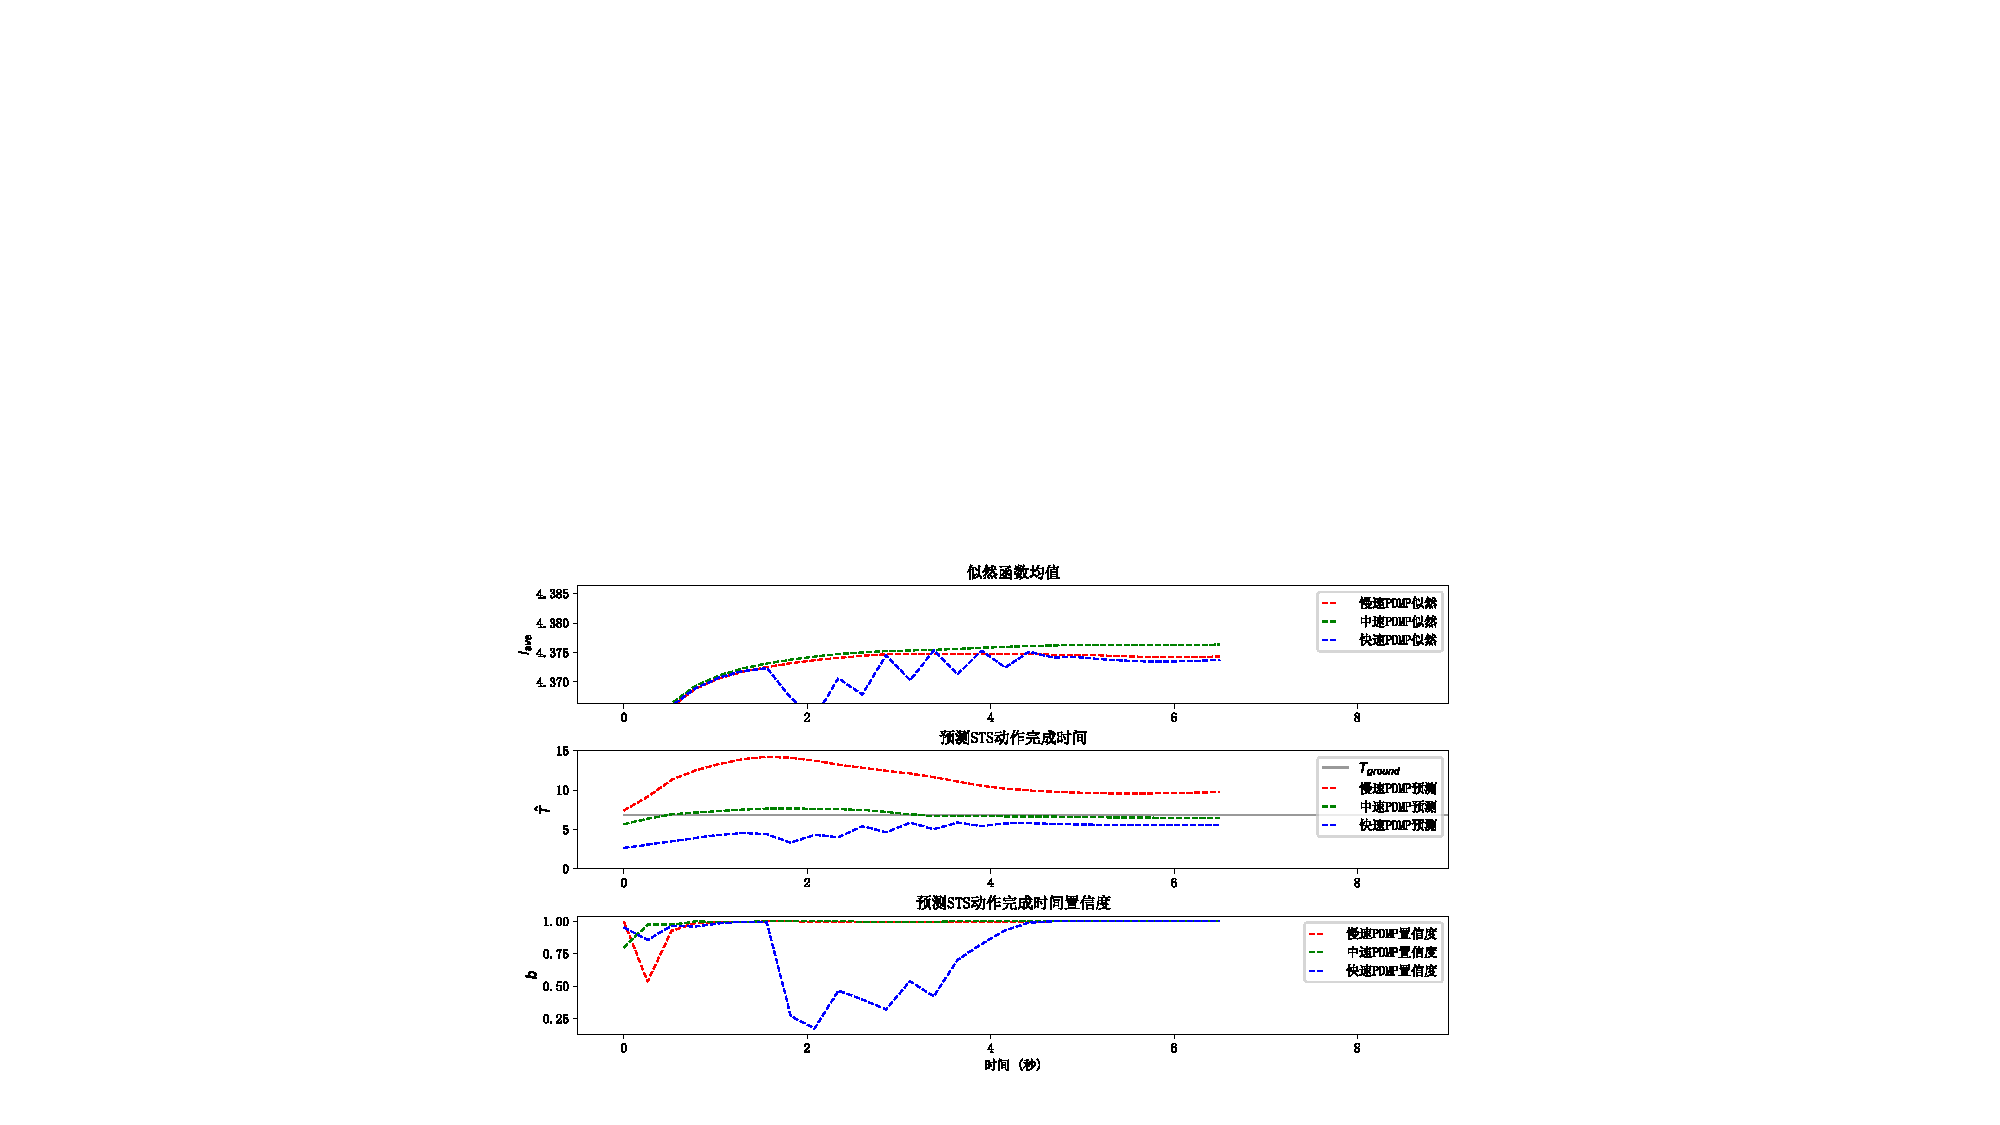
\includegraphics[width=1\textwidth]{figures/4-Fig-6.pdf}
    \caption{随着观测数据增多关于数据$l_{ave}$、$\hat T$以及$b$的变化曲线}
    \label{fig:4-6}
\end{figure}

\begin{figure}[htb]
    \centering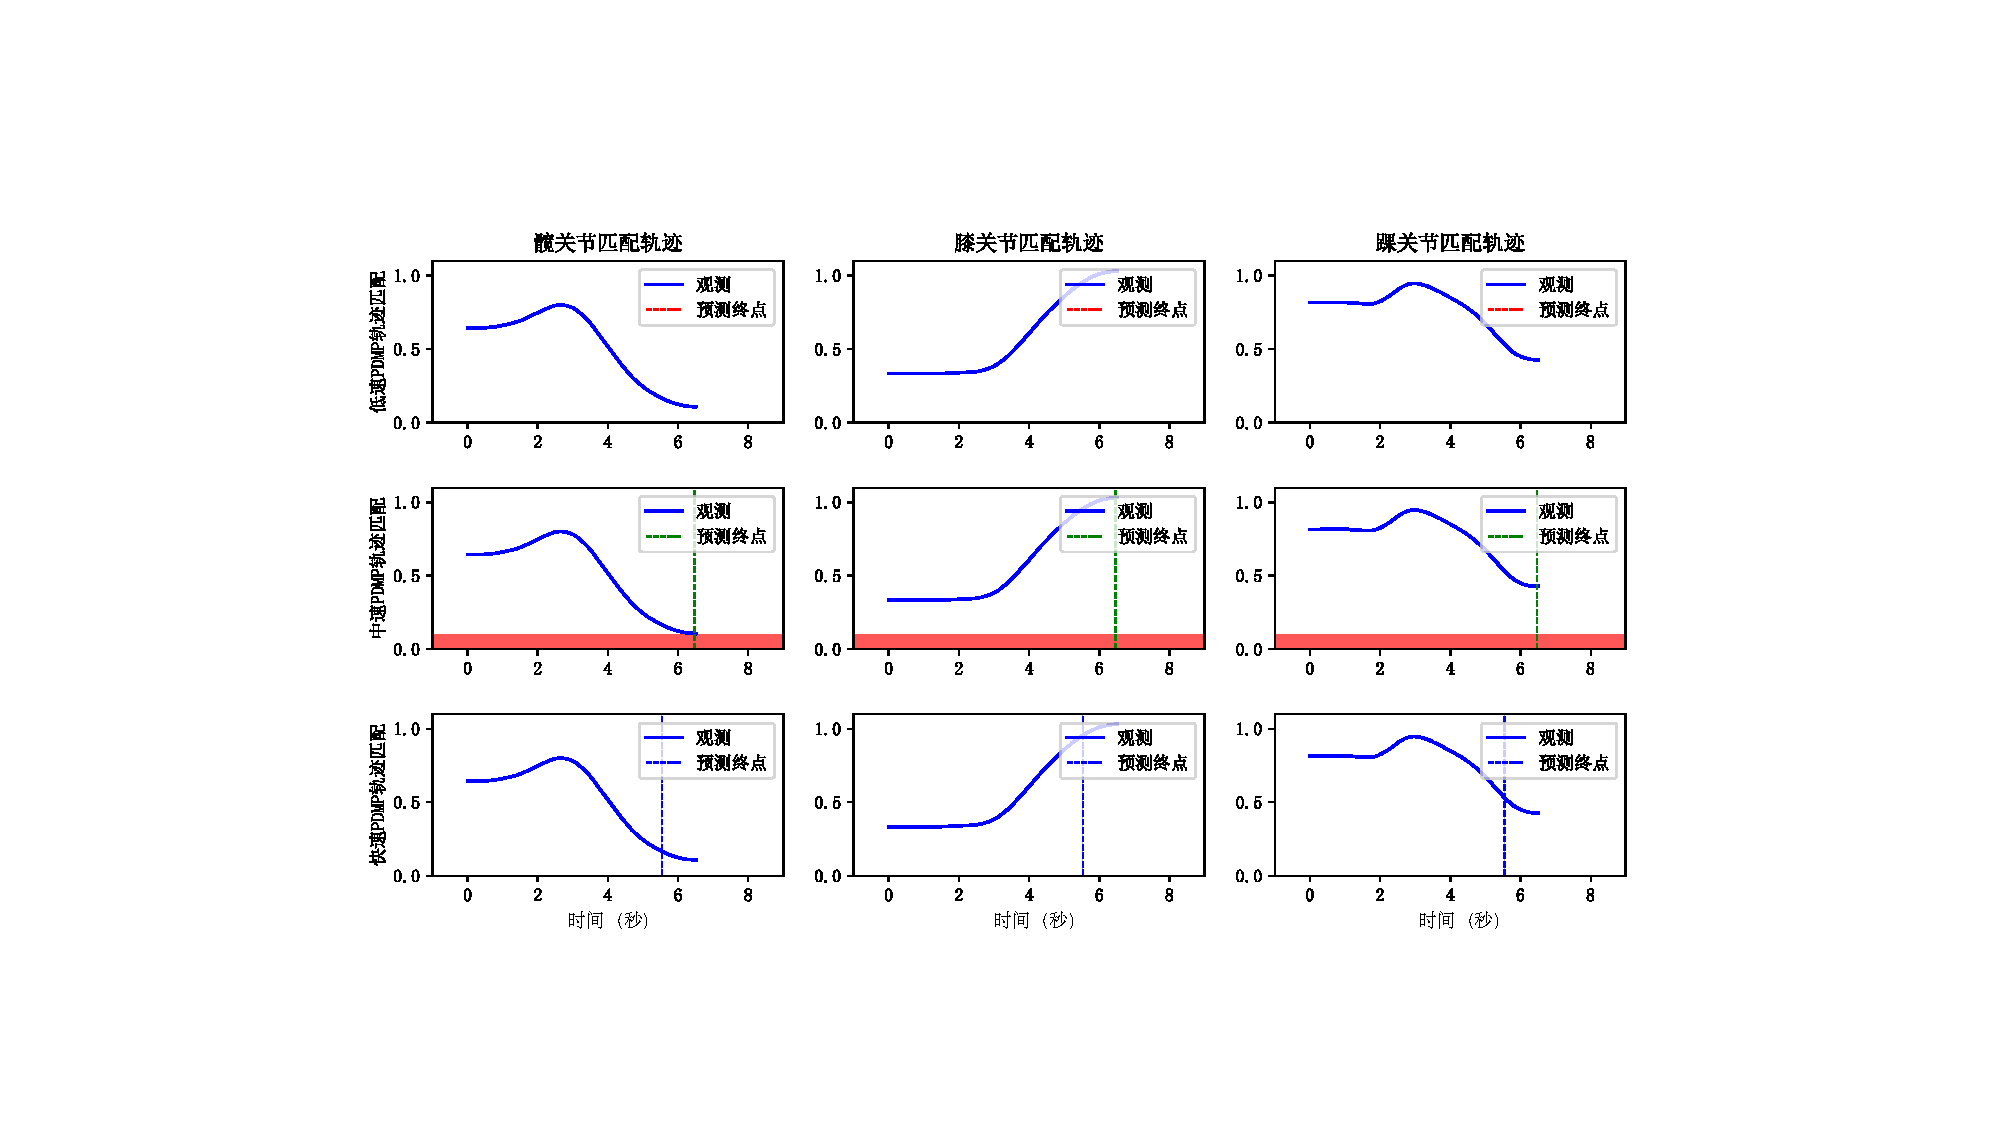
\includegraphics[width=1\textwidth]{figures/4-Fig-7.pdf}
    \caption{获得完全观测数据后生成的匹配轨迹和观测轨迹的对比,其中红色高亮表示当前选择的预测结果}
    \label{fig:4-7}
\end{figure}

在$t=1$时,由于获取的观测样本太少,EM优化算法无法积累足够多的``证据''推断出当前匹配的时间缩放系数$\tau$。此时,规划的轨迹主要基于$\tau$的初值生成,观测数据关于三个PDMP模型的平均似然$l_{ave}$都较低且没有区分度。三个模型关于预测的置信度$b$较低且存在较大幅度的波动,这表明当前数据不足导致EM的迭代优化还未收敛。因此,此时关于$\tau$的估计可信度较低,用于共享自主系统的仲裁函数将主要依赖于预定义值,以保证机器人系统的稳定性。在$t=2$时,随着获取的观测数据增多,慢速PDMP模型以及中速PDMP模型的优化过程趋于稳定地收敛,而快速PDMP的参数优化过程出现了震荡,导致对于其预测值的置信度大幅度降低。这是因为EM算法作为一种迭代优化算法只能在一定条件下能够保证收敛性,即当迭代次数趋于无穷大时,算法会收敛到一个局部极大值点。当数据不完全时,EM算法可能会陷入局部最优解,导致振荡。这也从侧面说明了采用多模型预测方法的优势,即针对同一个任务通过增加更细粒度的模型可以更好地处理数据分布特征,其能够更好地处理模型参数和结构的不确定性。此外,与观测数据匹配度更好的模型可以以更快的速度收敛,减少了需要迭代的次数,从而提供更可靠和高效的预测结果。在$t=4$后,由于获得接近完整运动70\%的观测数据,所有模型的参数优化都趋于稳定收敛,且预测结果具有高水平的置信度。但是中速PDMP具有最好的时间预测精度,相较于真值仅有约5\%的偏差,而慢速PDMP和快速PDMP模型的预测结果分别存在高达46\%和20\%的偏差。这也体现在图\ref{fig:4-5}以及在获得对于下肢STS运动的完全观测后图\ref{fig:4-7}中中速PDMP的匹配轨迹和观测数据最吻合,且在图\ref{fig:4-6}中可以看到中速PDMP的平均似然$l_{ave}$相较于其他两个模型更高。
\begin{table}[htb]
    \centering
    \caption{所提出方法在所构建坐立运动测试数据集上的表现}
    \setlength{\tabcolsep}{5pt}
    \begin{tabular}{c c c c}
    \hline\hline
     时间范围 & 成功预测/总轨迹数量 & 平均预测时间误差 & 成功预测所需的观测数据比例\\  
    \hline
    $2\backsim 4$秒& 9/12 & 7.3\%& 57\%\\ 
    $4\backsim 7$秒& 12/13 & 5.8\%& 53\%\\ 
    $7\backsim 10$秒& 5/5 & 5.1\%& 48\%\\ 
    \hline\hline
    \end{tabular}
    \label{tab:4-1}
\end{table}    

此外,基于所采集的测试运动数据集,对所提出方法进行运动时间预测的效果进行了分析。如表\ref{tab:4-1}所示。测试数据集中的运动轨迹时间持续长在2秒至10秒范围之间,我们根据持续时间将其分为了$2\backsim 4$、$4\backsim 7$以及$7\backsim 10$秒三个组别。当预测时间相较于真实值的误差低于10\%的阈值并保持1秒后或直至观测轨迹到达终点位置,则该次预测是成功的。此外,实现成功预测需要的观测轨迹比例定义为:从轨迹开始到进入阈值区间的时间长度与完整观测轨迹的长度之比。最终在$2\backsim 4$这一范围内STS运动有75\%被成功匹配和预测完成时间,相较于其他两个时间范围的92\%和100\%成功率,成功率较低的原因是其轨迹持续时间较短,在同等的传感系统观测频率下导致可用于EM迭代优化的数据更少导致的。由于轨迹持续时间短导致EM优化的迭代次数更少,对于$2\backsim 4$秒范围内的坐立运动,预测结果相较于真实完成坐立运动时间的平均预测误差达到7.3\%,高于其他两组持续时间更长的轨迹($4\backsim 7$秒:5.8\%和$7\backsim 10$秒:5.1\%)。在成功预测所需的观测数据所占全部数据的比例来看,三个时间段内的轨迹都具有相似的结果。这是因为在本任务中不同速度下的STS运动轨迹是在拓扑结构上相似的,例如在实验中我们发现,当运动轨迹出现变化并具有显著特征时,迭代优化的收敛速度会显著加快。当技能库中具有不同种类的动作时,关于成功预测所需的观测数据比例在不同任务中的表现有待进一步研究。

综合来看,所设计方法可以基于部分对于下肢关节运动的观测成功实现坐立动作完成时间的预测。基于先验知识库的多模型方法,对于提高轨迹运行时间预测的成功率以及精准度具有积极的作用。但是值得注意的是,当前的算法的时间复杂度是$O(N)$的,这表明随着观测数据的增加会导致每次进行EM优化的计算耗时会线性增长。因此该方法可能并不适用于需要累计长时间观测数据的在线运动时间推断。尽管使用性能更好的计算平台可以有效解决这一问题,但是如何降低计算时间复杂度仍然是今后的一个主要工作方向。

\section{本章小结}
本章节围绕站立功能辅助机器人应用中对于被辅助对象完成站立运动速度的不确定性自适应问题展开了研究。研究通过离散动态运动基元对人体下肢站立运动中的踝、膝、髋关节的运动轨迹进行了建模表征,并对其进行概率化处理。通过采集真实场景下的人体坐立离线运动数据,建立了一个包含快速、中速、慢速运动轨迹模板的先验技能库。为了实现根据当前部分对被辅助对象的观测实在线坐立运动时间估计,本章研究将运动时间意图估计问题看作一个系统参数辨识问题,基于期望最大化算法实现了部分观测下的连续运动时间估计。此外,所设计交互意图估计方法通过一个置信度水平量化指标可以嵌入一个共享自主系统中,在保证机器人个体适应性的同时实现安全可靠的辅助机器人的在线运动轨迹优化。
